\documentclass[notes]{beamer}
\usetheme{Madrid}
\usepackage[utf8]{inputenc}
\usepackage{lmodern}
\usepackage{scrextend}
\usepackage{bbding}
\usepackage{color}
\changefontsizes{8pt}

%%%%%%%%%%%%%%%%%%%%%%%%%%%%%%%%%%%%%%%%%%%%%%%%%%%%%%%%%%%%%%%%%%%%%%%%%%%%%%%
% items enclosed in square brackets are optional; explanation below
\title{A screen space GPGPU surface LIC algorithm for parallel interactive exploration of large composite datasets}
\subtitle{Astronum 2014}
\author[Loring, Karimabadi, Roytershteyn, Daughton] % (optional, for multiple authors)
{\footnotesize B.~Loring~LBNL, H.~Karimabadi and V.~Roytershteyn~UCSD, W.~Daughton~~LANL} %
%\institute[Lawrence Berkeley National Laboratory] % (optional)
%{ \inst{1}LBNL, \inst{2}UCSD, \inst{3}LANL}
\date{\today}
%%%%%%%%%%%%%%%%%%%%%%%%%%%%%%%%%%%%%%%%%%%%%%%%%%%%%%%%%%%%%%%%%%%%%%%%%%%%%%%
% {
%\setbeamerfont{title}{family=\sf,size=\Huge}
%\setbeamertemplate{background canvas}{
\includegraphics[width=\paperwidth,height=\paperheight]{./title_page_bg.png}}
% \begin{frame}
%   \titlepage
% \end{frame}
%
% }
%\setbeamertemplate{background canvas}{
\includegraphics[width=\paperwidth,height=\paperheight]{./slide_bg.png}}
%\setbeamerfont{frametitle}{family=\sf,size=\Huge}


\begin{document}
\setbeamertemplate{enumerate items}[default]


\frame{\titlepage}

%==============================================================================
\begin{frame}{Introduction}
  \vspace{-0.1in}
  \begin{beamerboxesrounded}{Goal of the work}
  We set out to design a surface LIC algorithm that:
  \begin{enumerate}
  \item handles all common datasets, including AMR, multiblock etc...
  \item is parallel, can process large simulation data
  \item deployable in existing vis tools
  \item delivers interactive performance
  \item is flexible enough to work well on wide range of data
  \item exposes tuning parameters to the user
  \end{enumerate}
  \end{beamerboxesrounded}
  \end{frame}
% \note{}

%==============================================================================
\begin{frame}{Introduction}
  \vspace{-0.1in}
  \begin{beamerboxesrounded}{Surface LIC}
  \begin{center}
  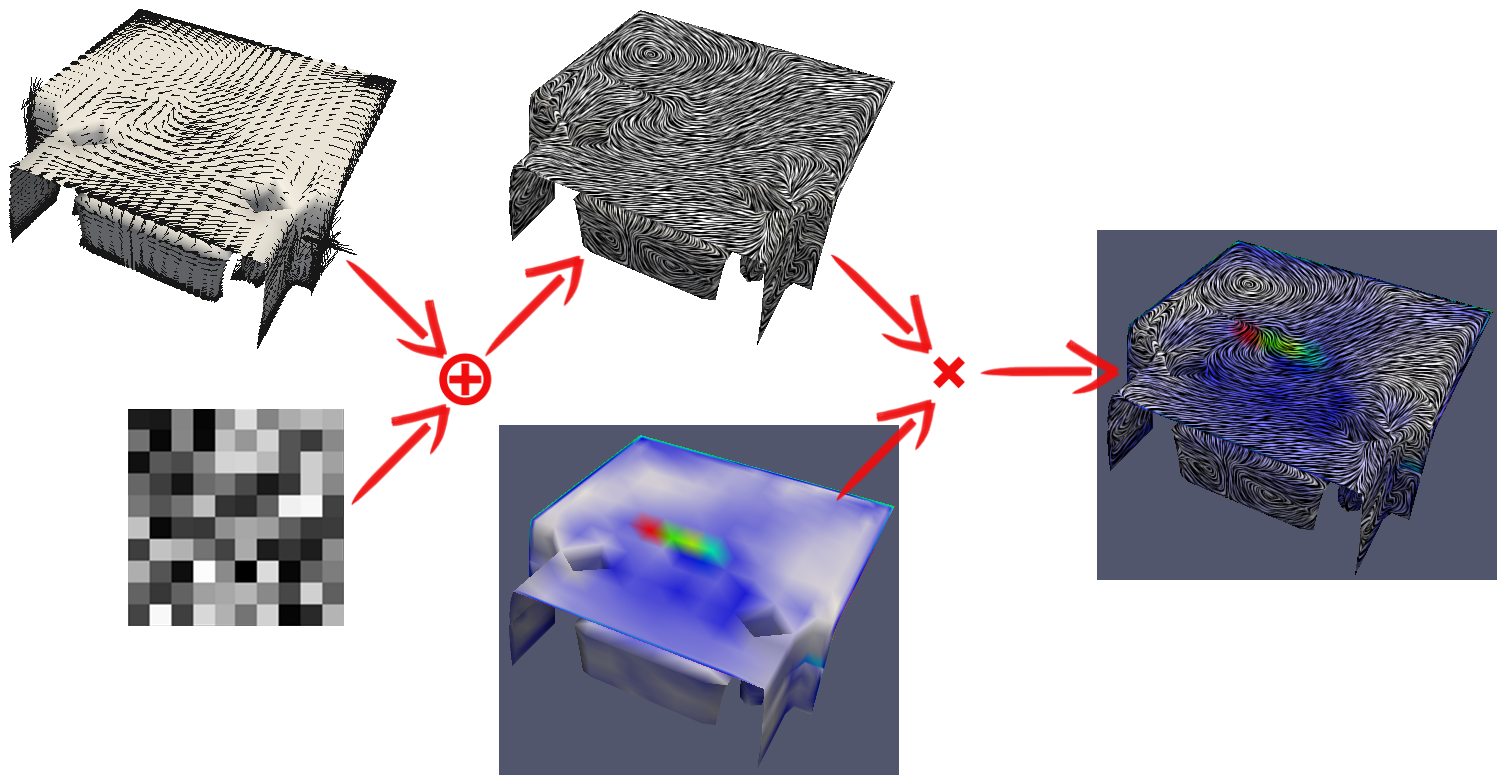
\includegraphics[width=4.75in]{office-all-4.png}\vspace{0.05in}\\
  {\footnotesize Noise $\otimes$ Surface Vectors = Surface LIC}
  \end{center}
  \end{beamerboxesrounded}
  \end{frame}
\note{
\scriptsize
* global view of the vector field, easily identify features \\
* computationally costly, GPGPU implementatation to make it interactive \\
* working in screen space introduces some interesting complexity and challenges \\
* especially for the parallelization, if you expect it to work in existing parallel vis tools \\
}

%==============================================================================
\begin{frame}{Introduction}
  \begin{beamerboxesrounded}{Screen space algorithm in detail}
  \begin{center}
    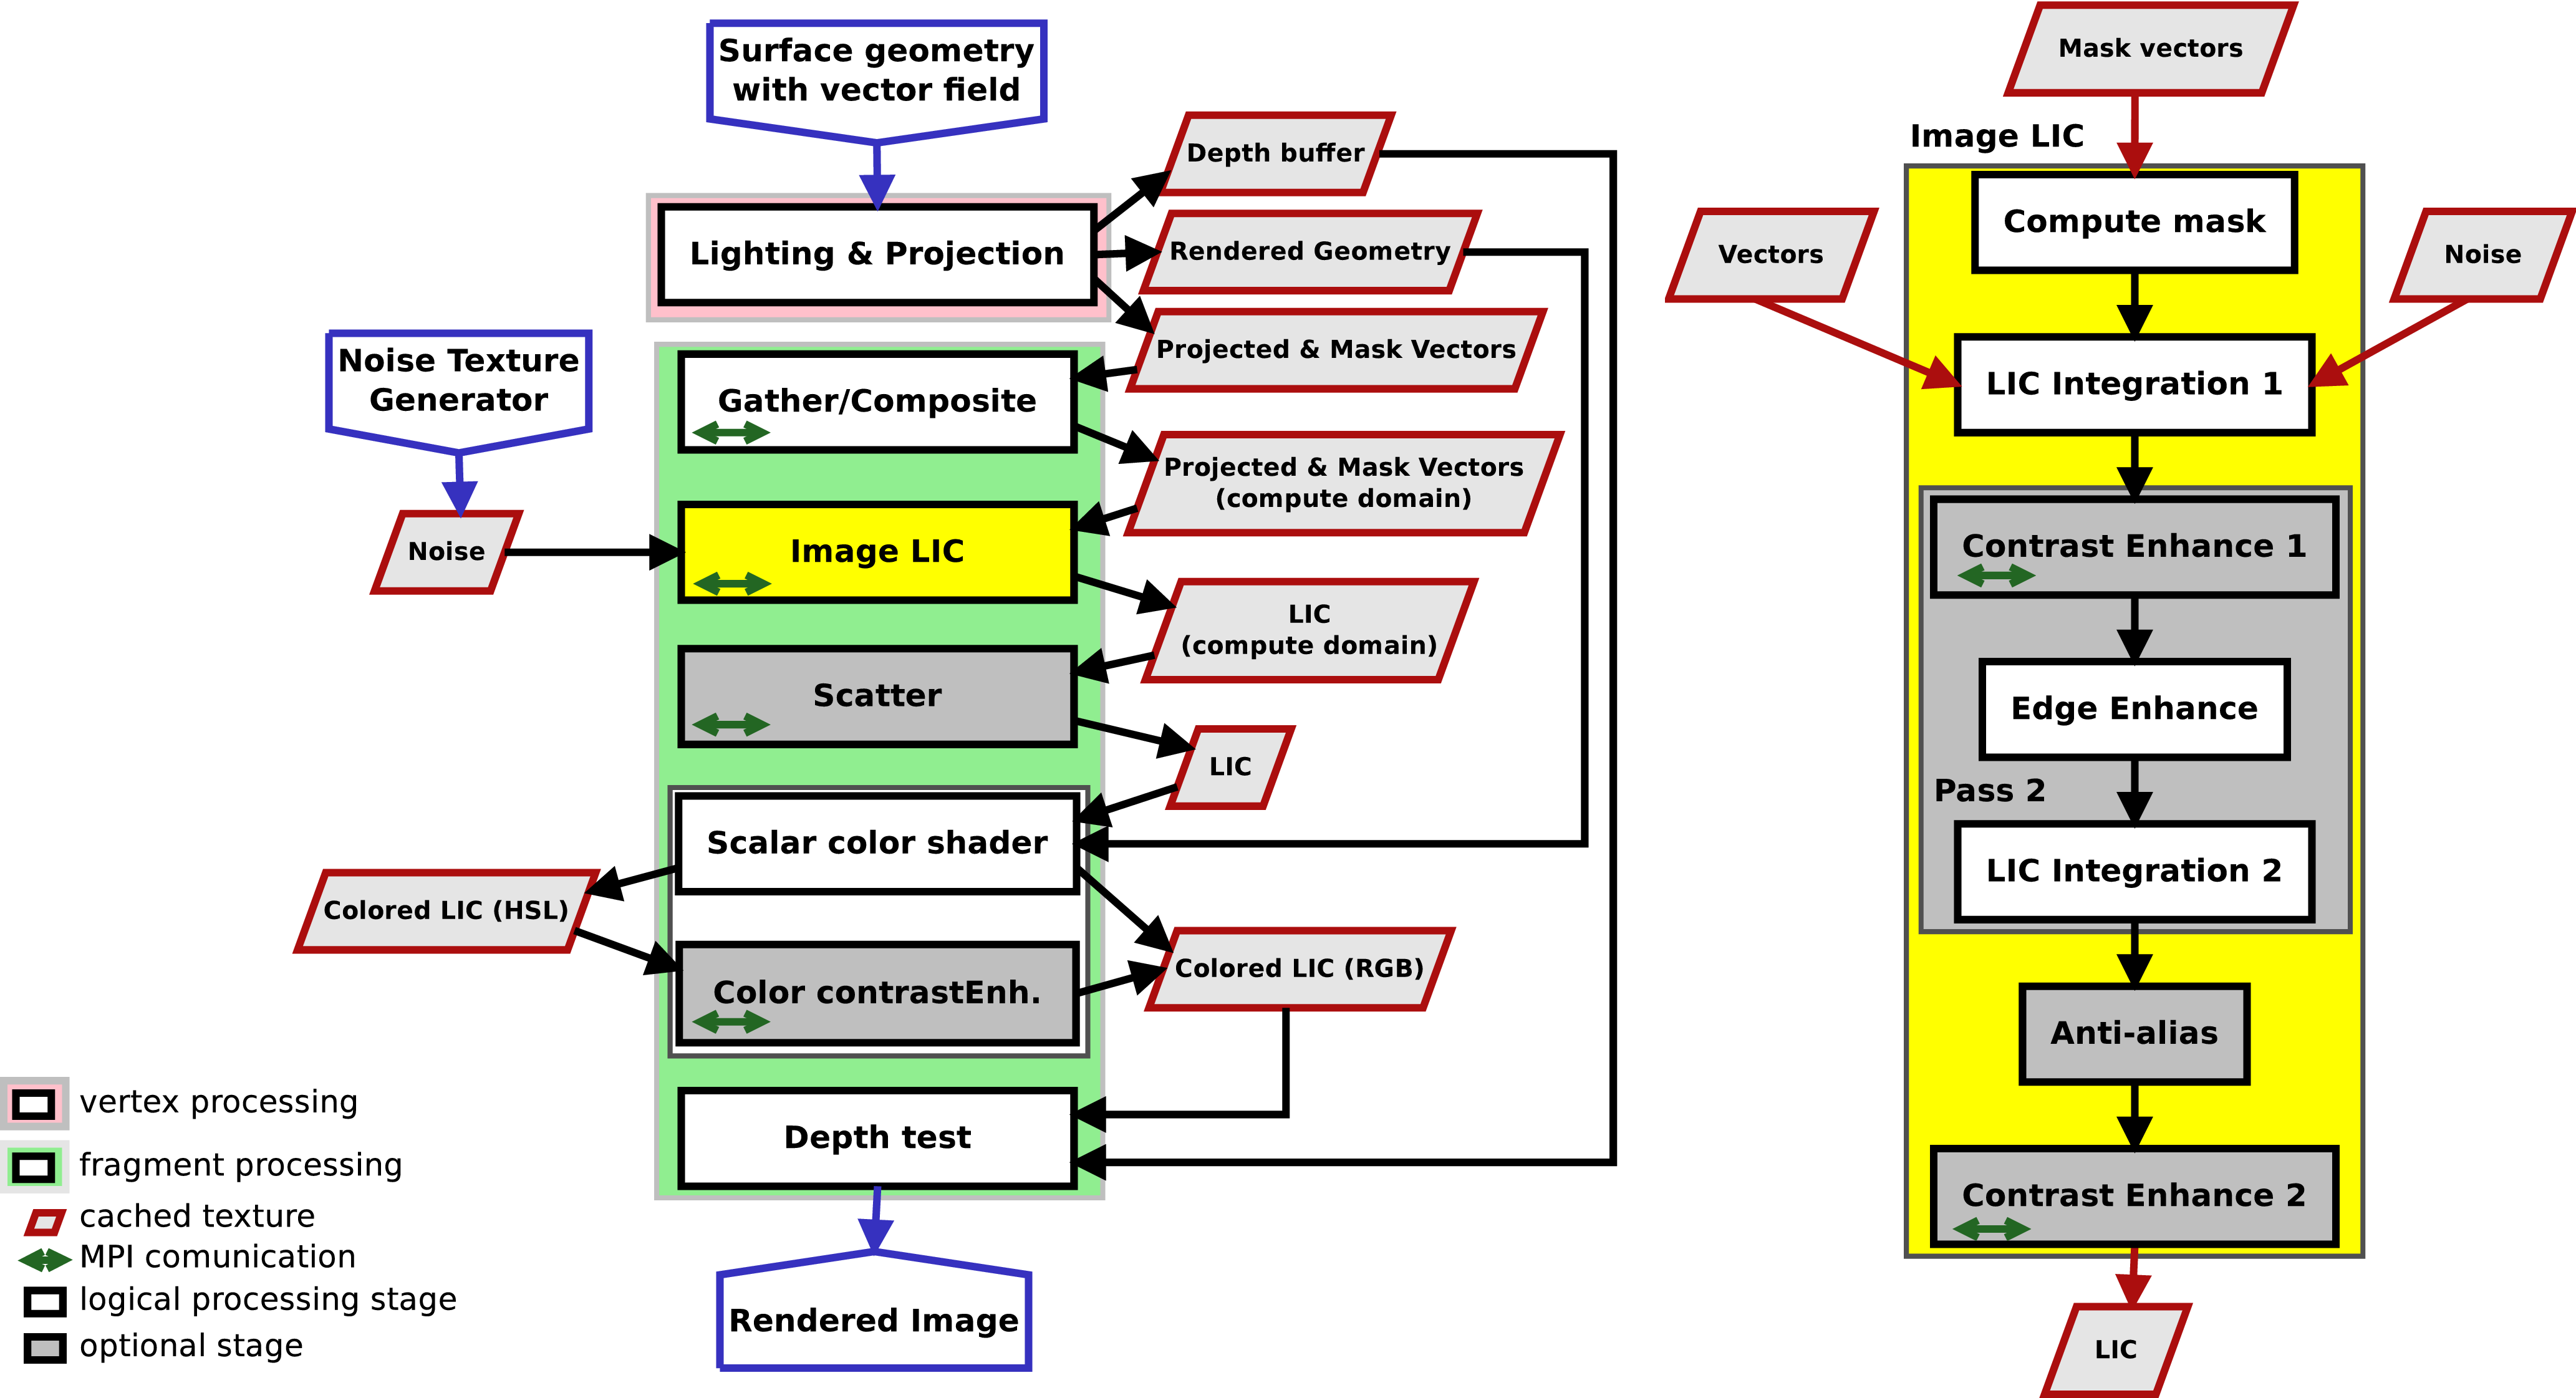
\includegraphics[width=4.2in]{flow-color.png}
  \end{center}
  \end{beamerboxesrounded}
  \end{frame}
\note{
\scriptsize
* lighting and projection shader
* screen space after this
* compositing stages for parallel 
* image LIC is broken out on the right
* 2 pass image LIC, first pass convolves noise, second pass convolves first pass after image processing filters
* some of the image processing stages require guard pixels for correct parallel operations
* some require reduction
* shaders for combining LIC and rendered geometry
* stages are cached
* works with IceT image compositing library used by ParaView and VisIt
}

%==============================================================================
\begin{frame}{Parallelization}

  \begin{beamerboxesrounded}{Typical sort-last redering}
      \begin{center}
      \raisebox{-0.5\height}{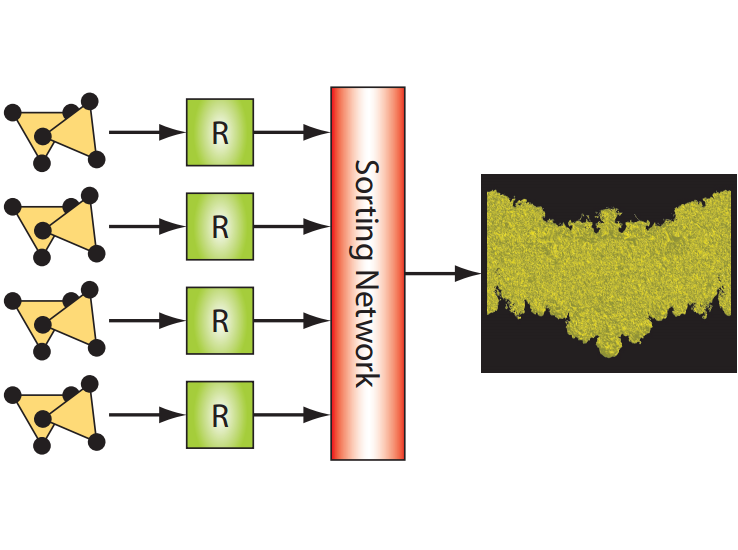
\includegraphics[height=1.75in]{render-sorting.png}}\hspace{0.1in}
      \raisebox{-0.5\height}{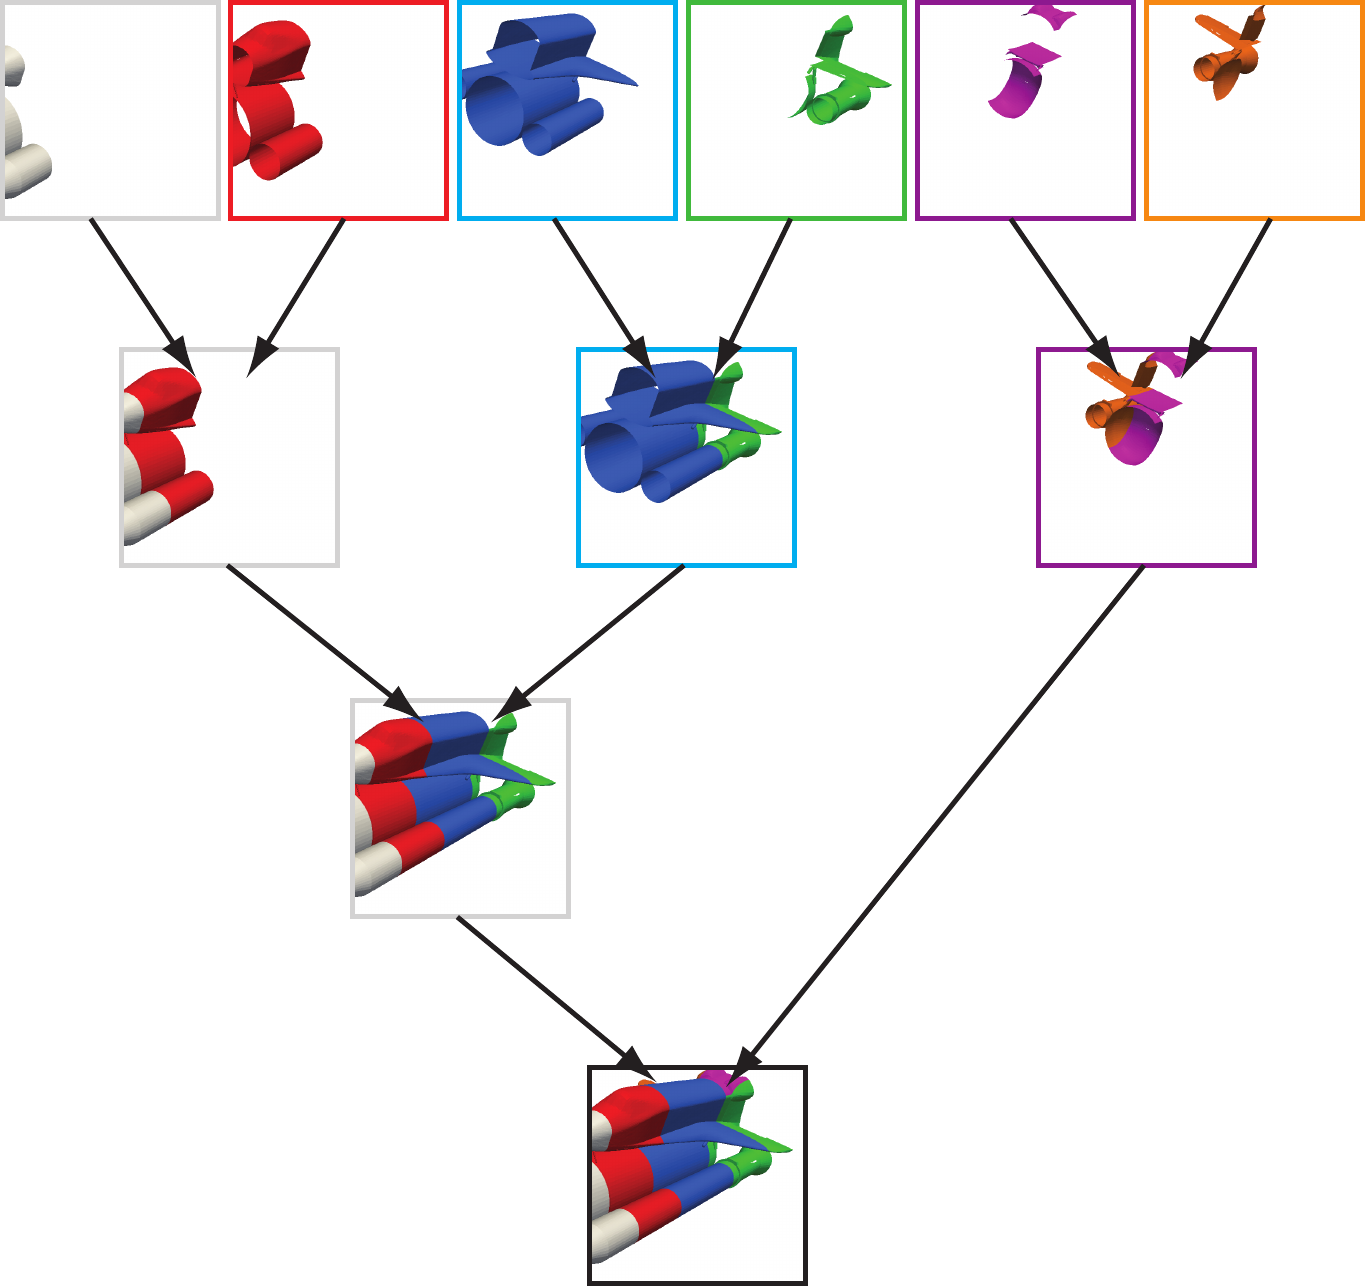
\includegraphics[height=1.5in]{icet-tree-composite.png}}
      \end{center}
      \vspace{-0.15in}
      \begin{itemize}
      \scriptsize
      \item Render geometry distributed. z-buffer compositing reduction to rank 0 selects visible data. image delivery.
      \item Typically simulation domain decomp is used. Pixels processed where the lie. Fine rendering is typically fast compared to I/O and processing.
      \item Sorting is done in screen space. communication pattern depends on view paramters.
      \item We're working with the IceT compsiting library used by ParaView and VisIt.
      \end{itemize} 
  \end{beamerboxesrounded}
\end{frame}
\note{\scriptsize
distributed geometry using simulation domain decomp \\
screen space domain decomposition is view dependent \\
cloesest pixels need to be displayed thus z-buffer compositing\\
}


%==============================================================================
\begin{frame}{Parallelization}
  \begin{beamerboxesrounded}{Sort last with screen space surface LIC}
      \begin{center}
      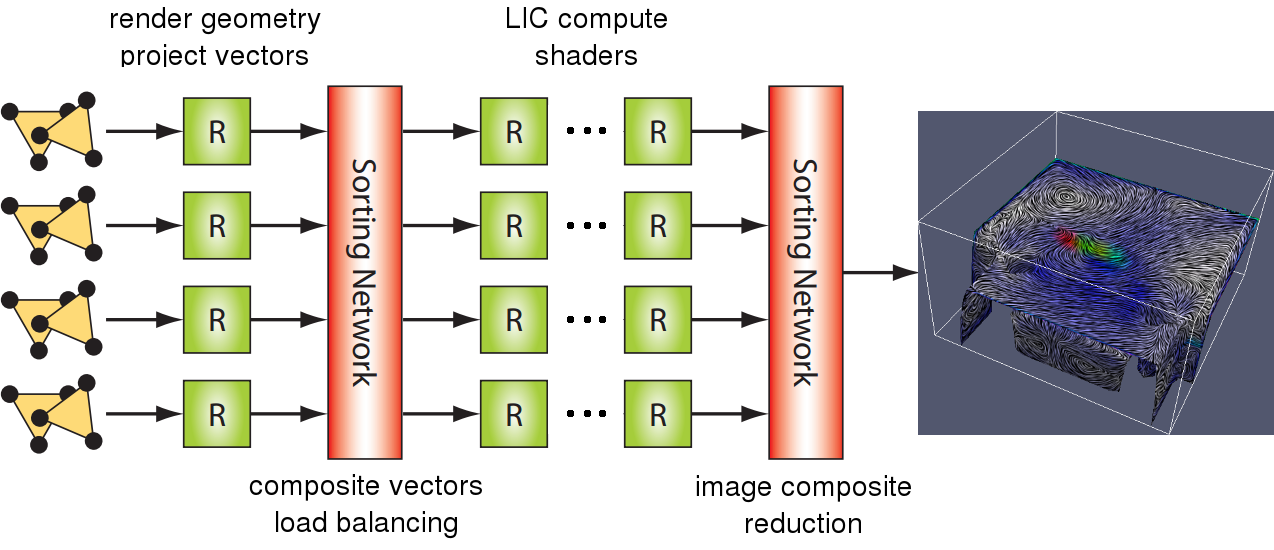
\includegraphics[height=1.75in]{render-sorting-plus-lic.png}
      \end{center}
      \vspace{-0.15in}
      \begin{itemize}
      \item prior to integration composite vectors where screen space projections overlap
      \item need ``guard pixels'' at screen space block boundaries
      \item shader communication, eg. to get min/max for histogram stretching
      \end{itemize} 
  \end{beamerboxesrounded}
\end{frame}

%==============================================================================
\begin{frame}{Parallelization}
  \begin{beamerboxesrounded}{Communication stages}
  \begin{center}
    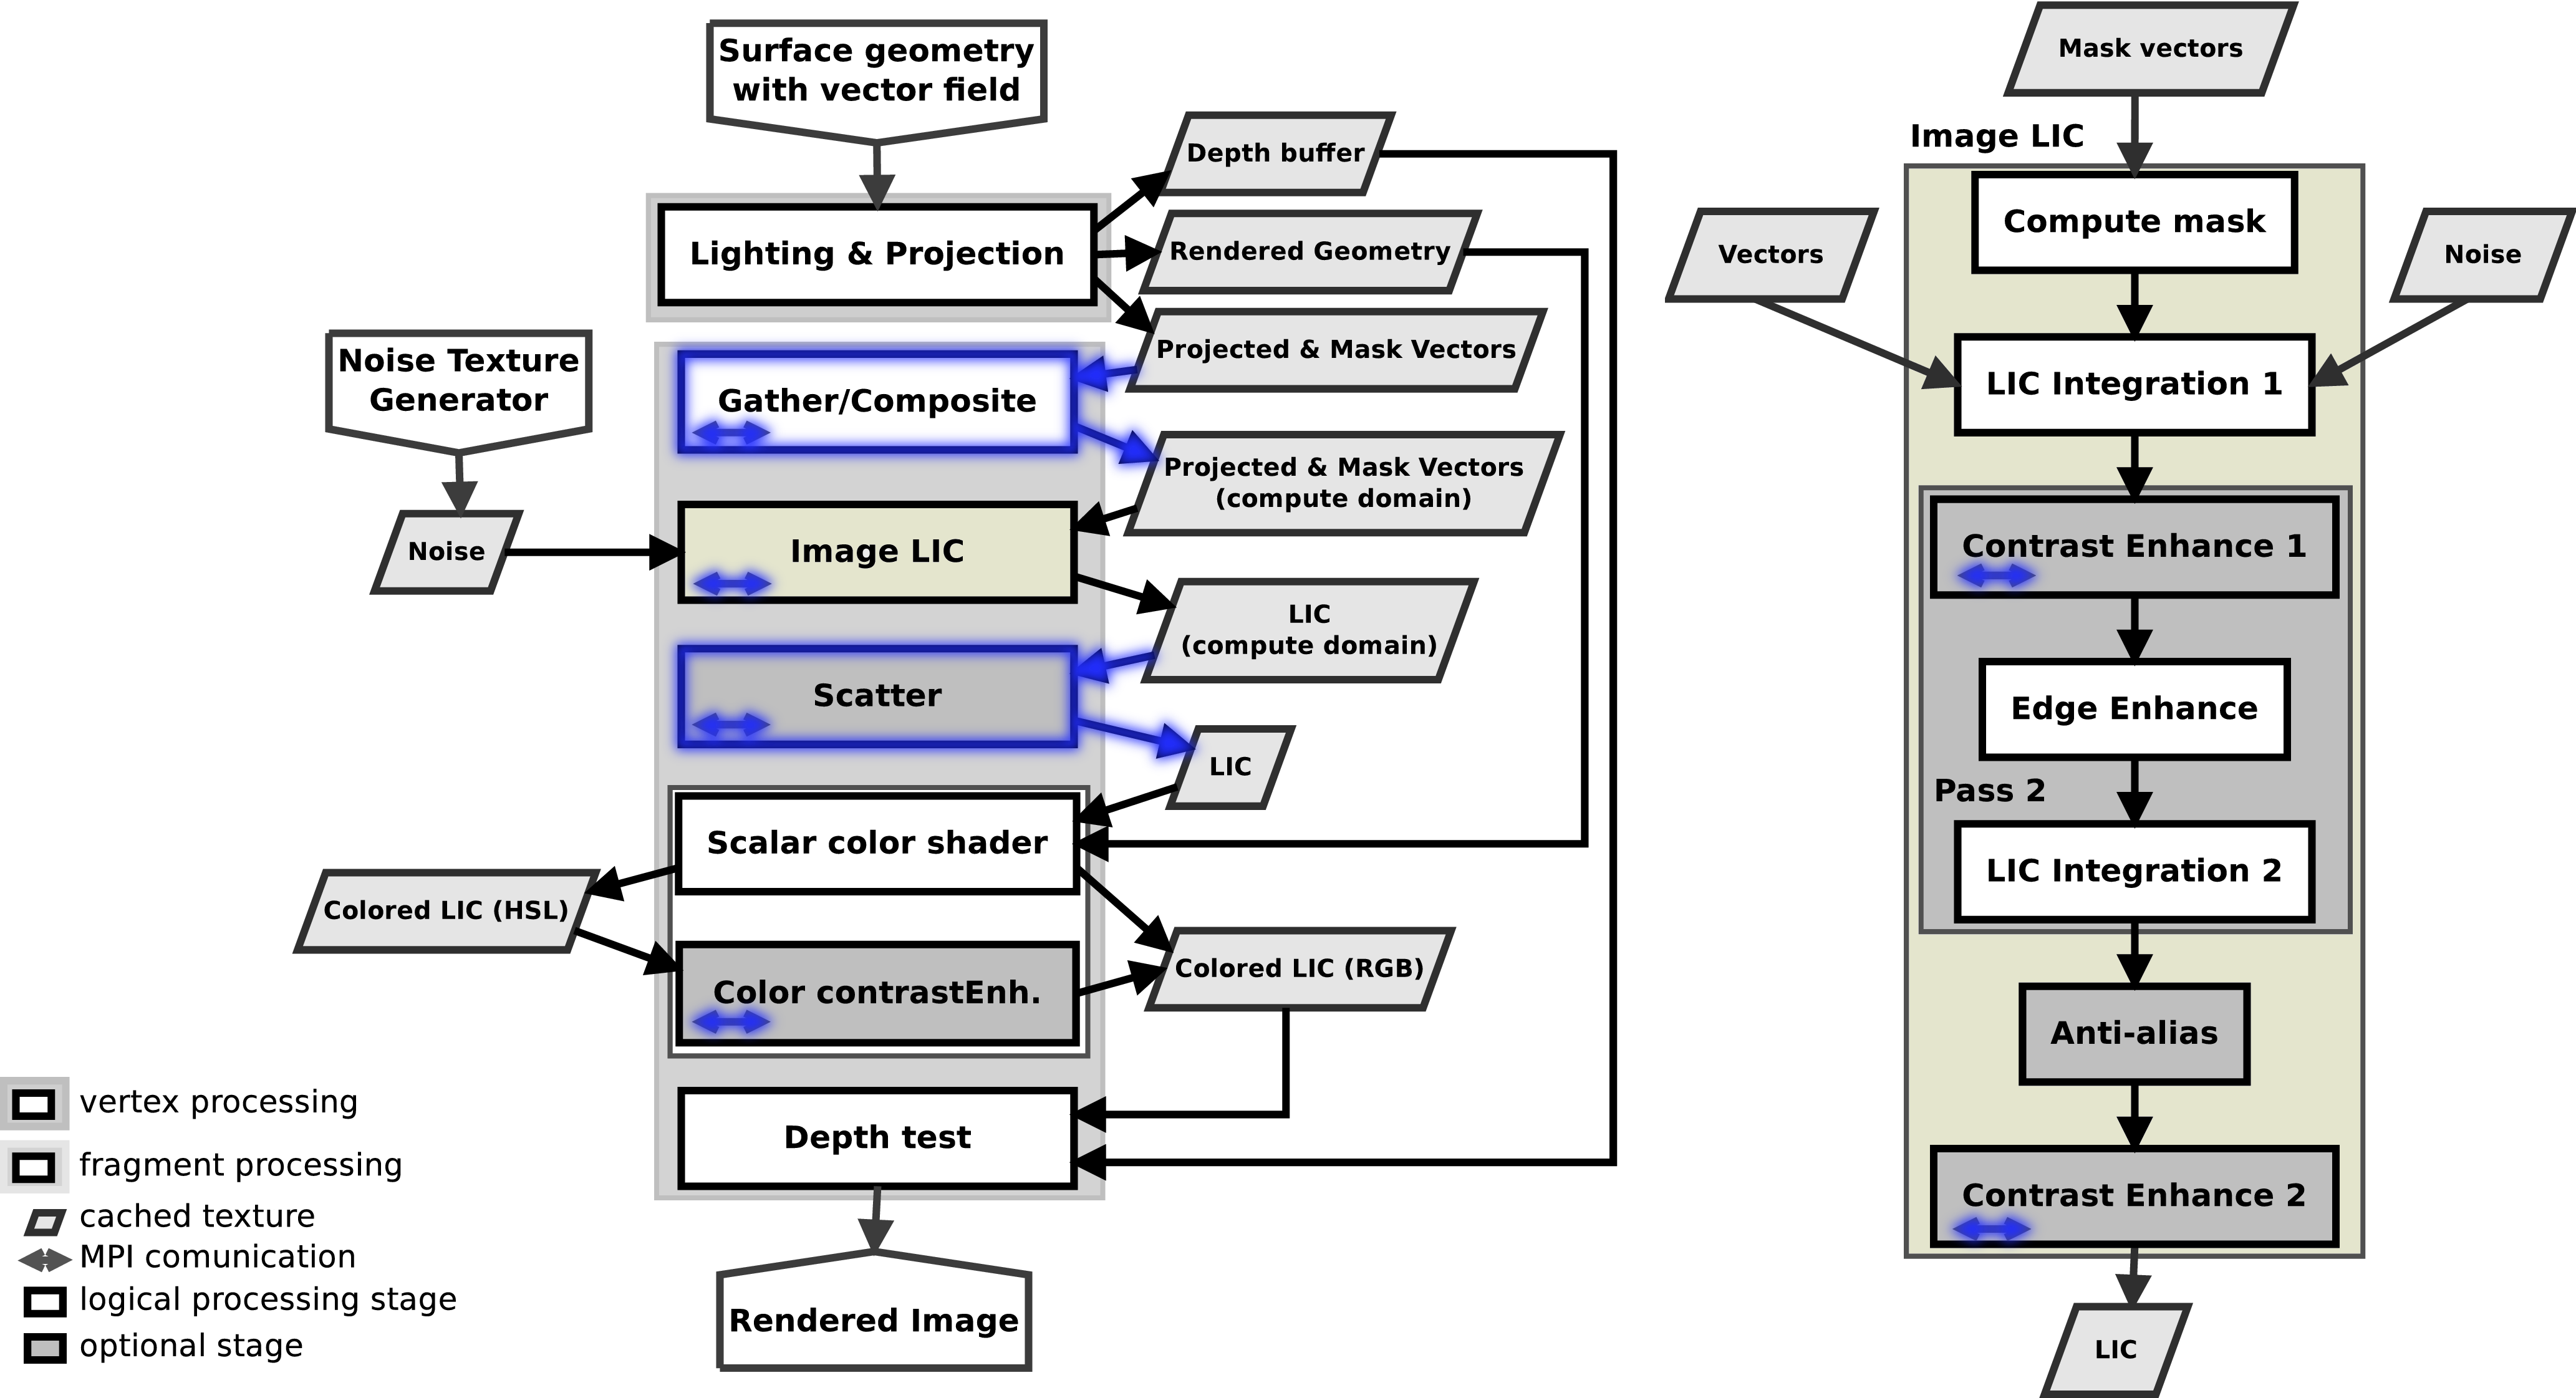
\includegraphics[width=4.2in]{ce-flow-par.png}
  \end{center}
  \end{beamerboxesrounded}
  \end{frame}

\note{\scriptsize
* compositing + ghost generation done in the gather stage
* image processing stages need min/max
* scatter is a transfer only op, no compositing
* scatter stage is needed *if* we do any screen space load balancing because IceT pre-computes the image space bounds
* this could be addressed so that the scatter is not needed, but then we need to composite color buffer so its actually not that bad
}

%==============================================================================
\begin{frame}{Parallelization}
\vspace{-0.05in}
\begin{beamerboxesrounded}{Working in screen space}
  \begin{center}
  \only<1>{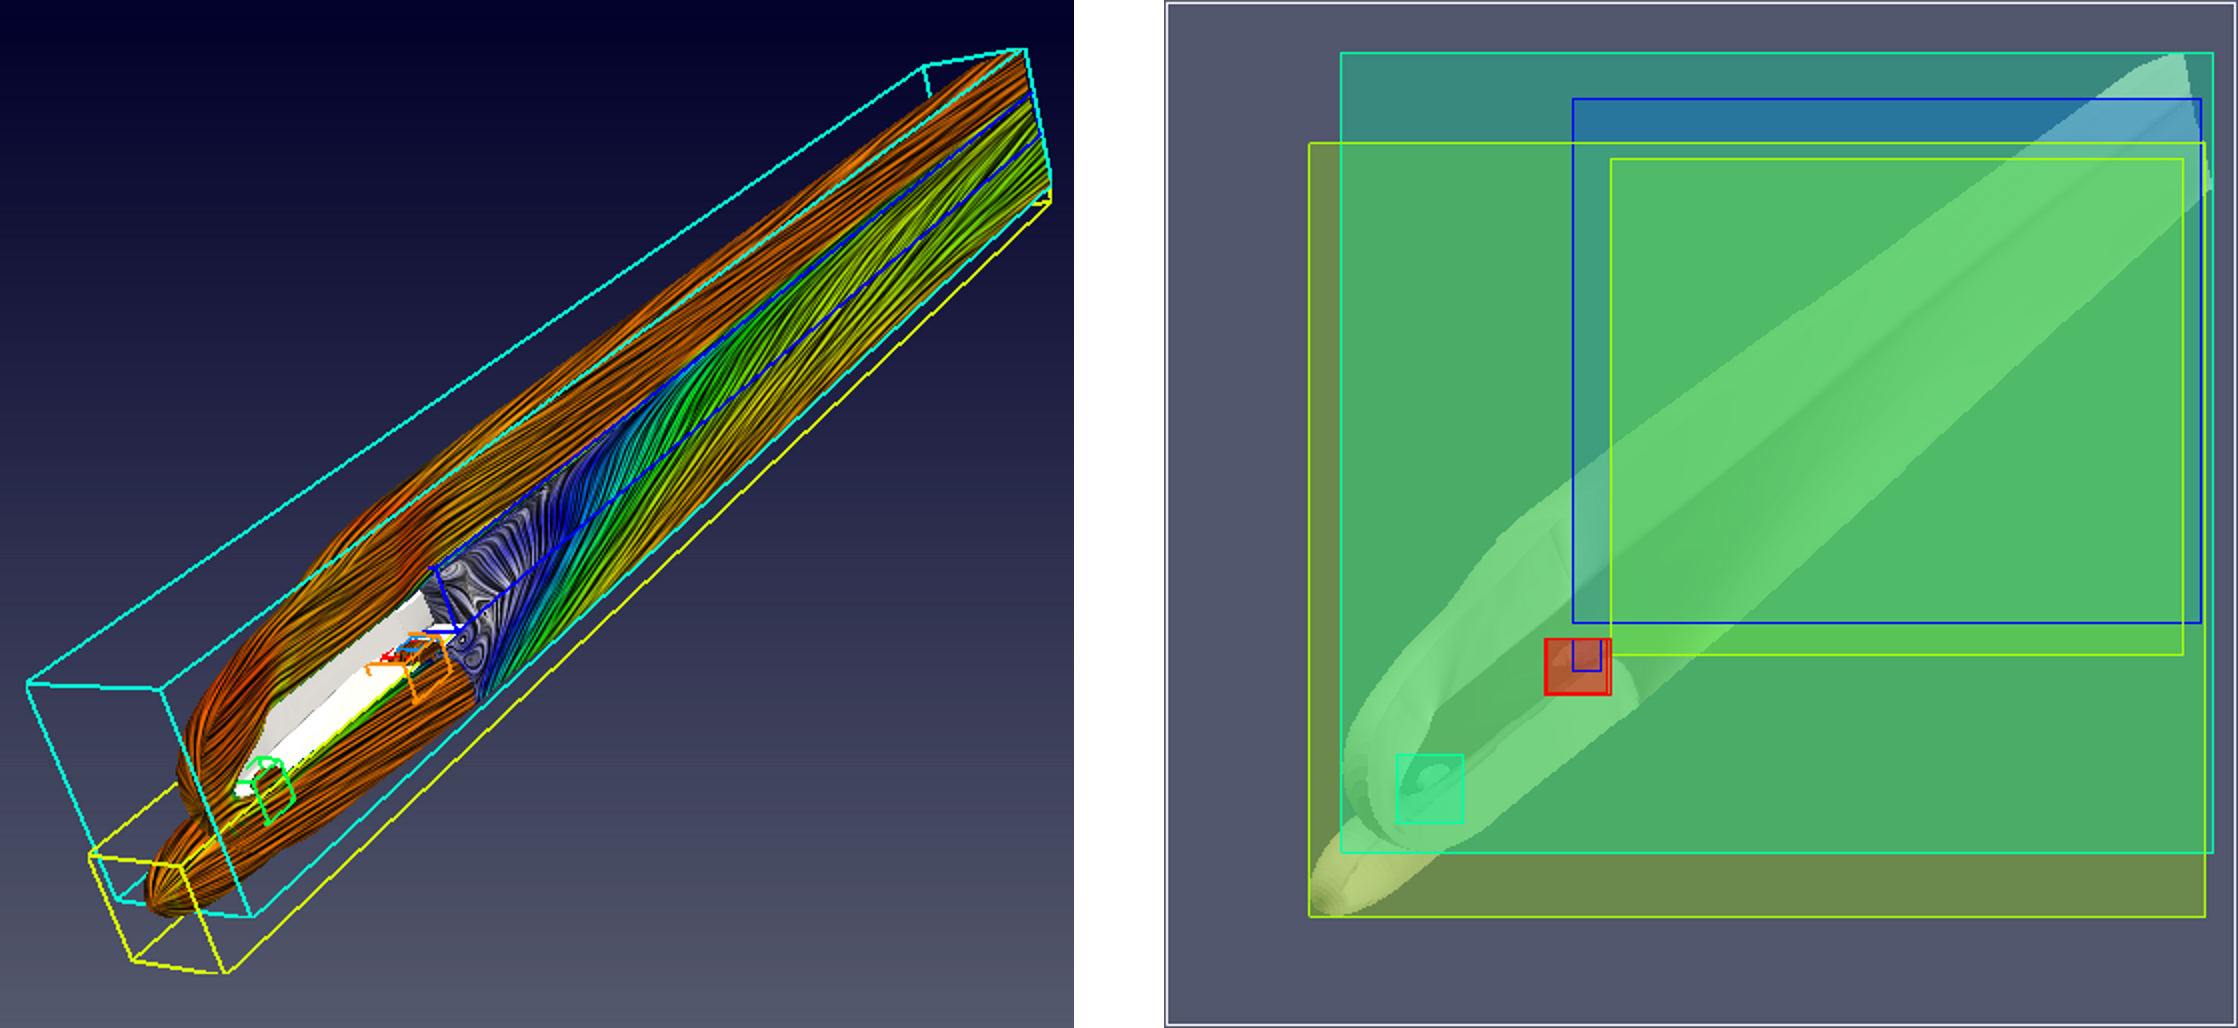
\includegraphics[width=3.7in]{shuttle-inplace.png}}
  \only<2>{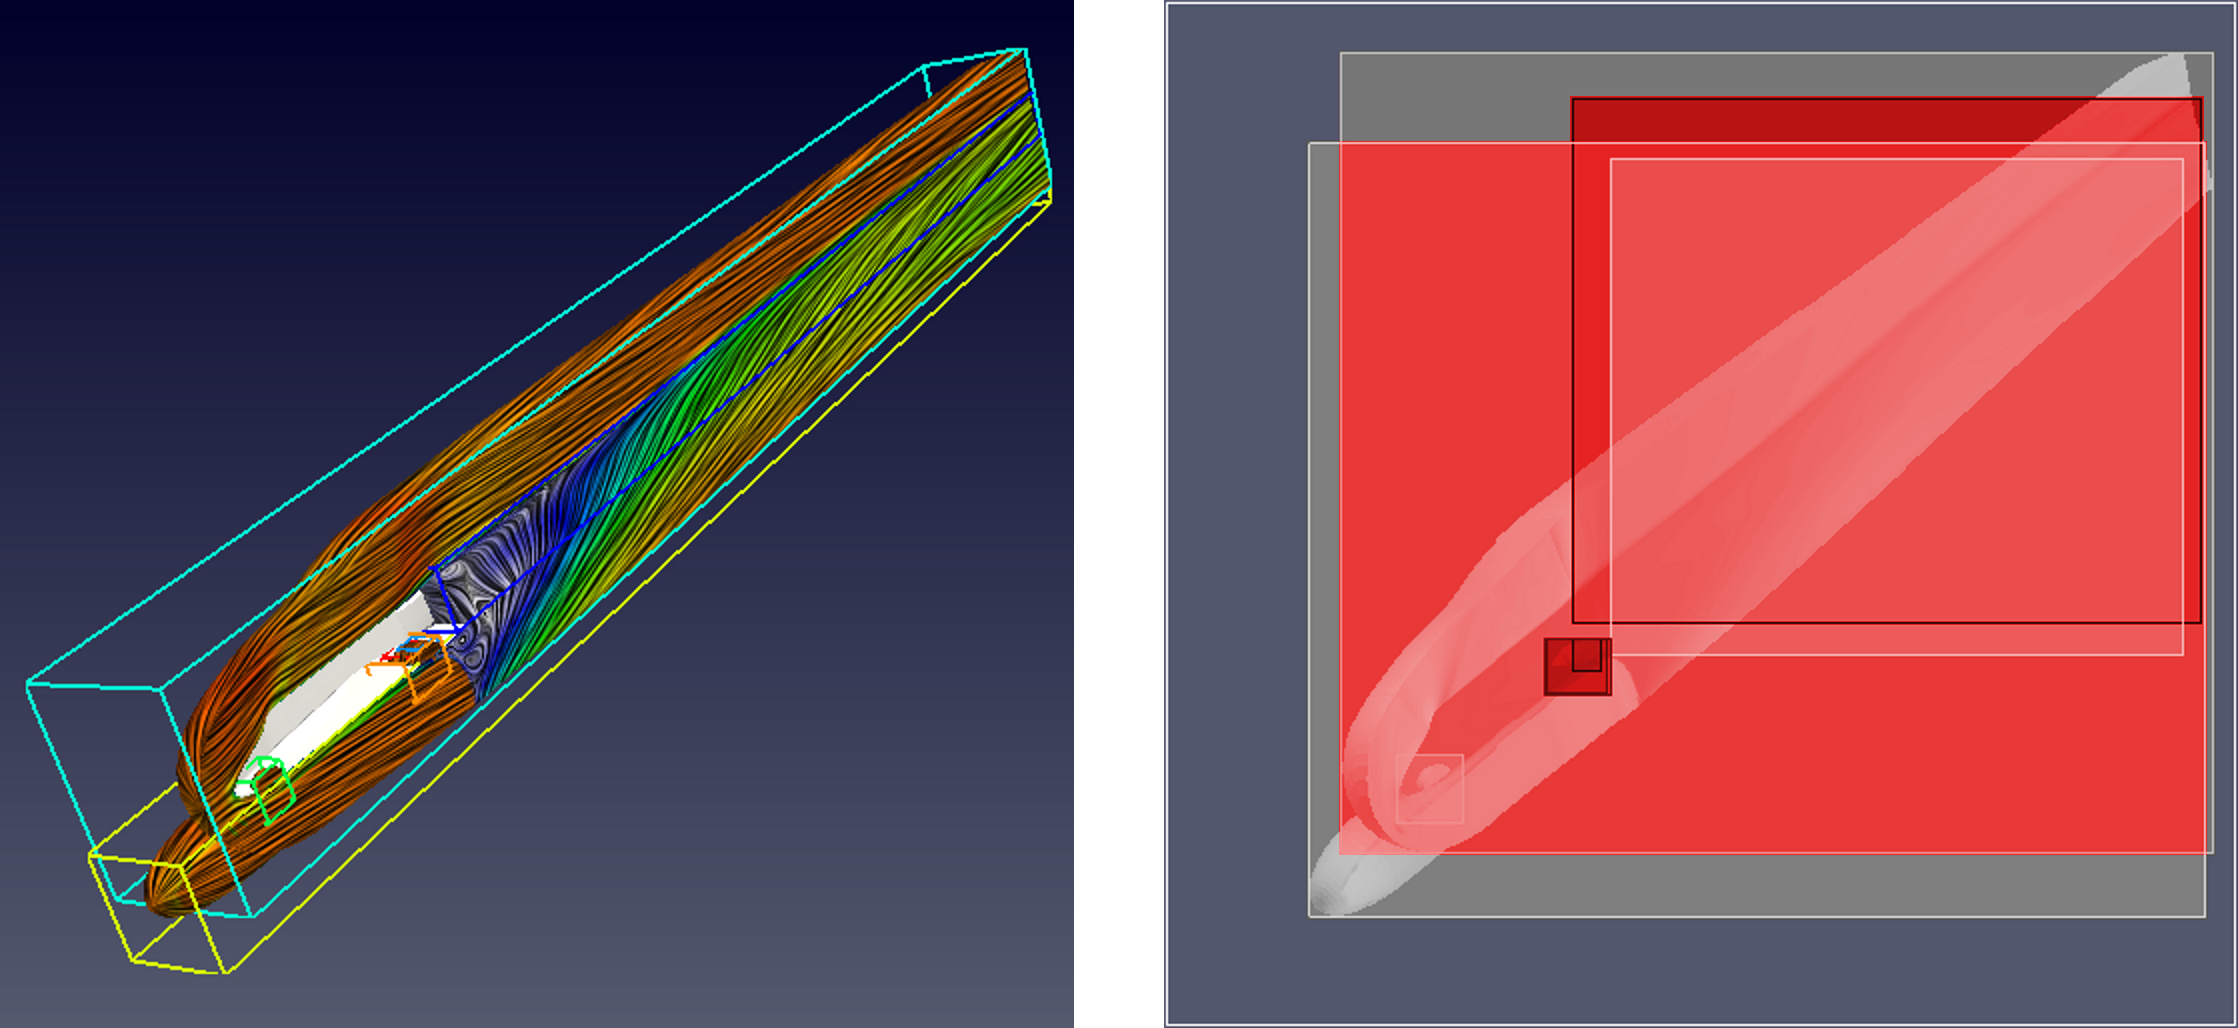
\includegraphics[width=3.7in]{shuttle-inplace-red.png}}
  \end{center}
  \vspace{-0.15in}
  \begin{description}
  \item [In-place Composite]Lazy. Process on the existing screen space extents.
  \end{description}
  \vspace{-0.1in}
  \begin{minipage}{0.5\linewidth}
  \begin{itemize}
  \setlength{\itemindent}{-1em}
  \footnotesize 
  \item[\color{green}{\Checkmark}] Simple, works with IceT
  \item[\color{green}{\Checkmark}] It's the best if there's no overlap (ie slice)
  \only<2>{\item[\color{red}{\XSolidBrush}] view dependent/not load balanced}
  \end{itemize}
  \end{minipage}
  \begin{minipage}{0.5\linewidth}
  \only<2>{
  \begin{itemize}
  \setlength{\itemindent}{-1em}
  \footnotesize 
  \item[\color{red}{\XSolidBrush}] high communication costs. all process pairs with overlapping regions exchange data
  \item[\color{red}{\XSolidBrush}] redundant computation can limit performance
  \end{itemize}
  }
  \end{minipage}
  \only<2>{\begin{center}\color{red}{\bf \it screen-space overlap is costly!!}\end{center}}
  \end{beamerboxesrounded}
\end{frame}


%==============================================================================
\begin{frame}{Parallelization}
  \vspace{-0.05in}
\begin{beamerboxesrounded}{Working in screen space}
  \begin{center}
  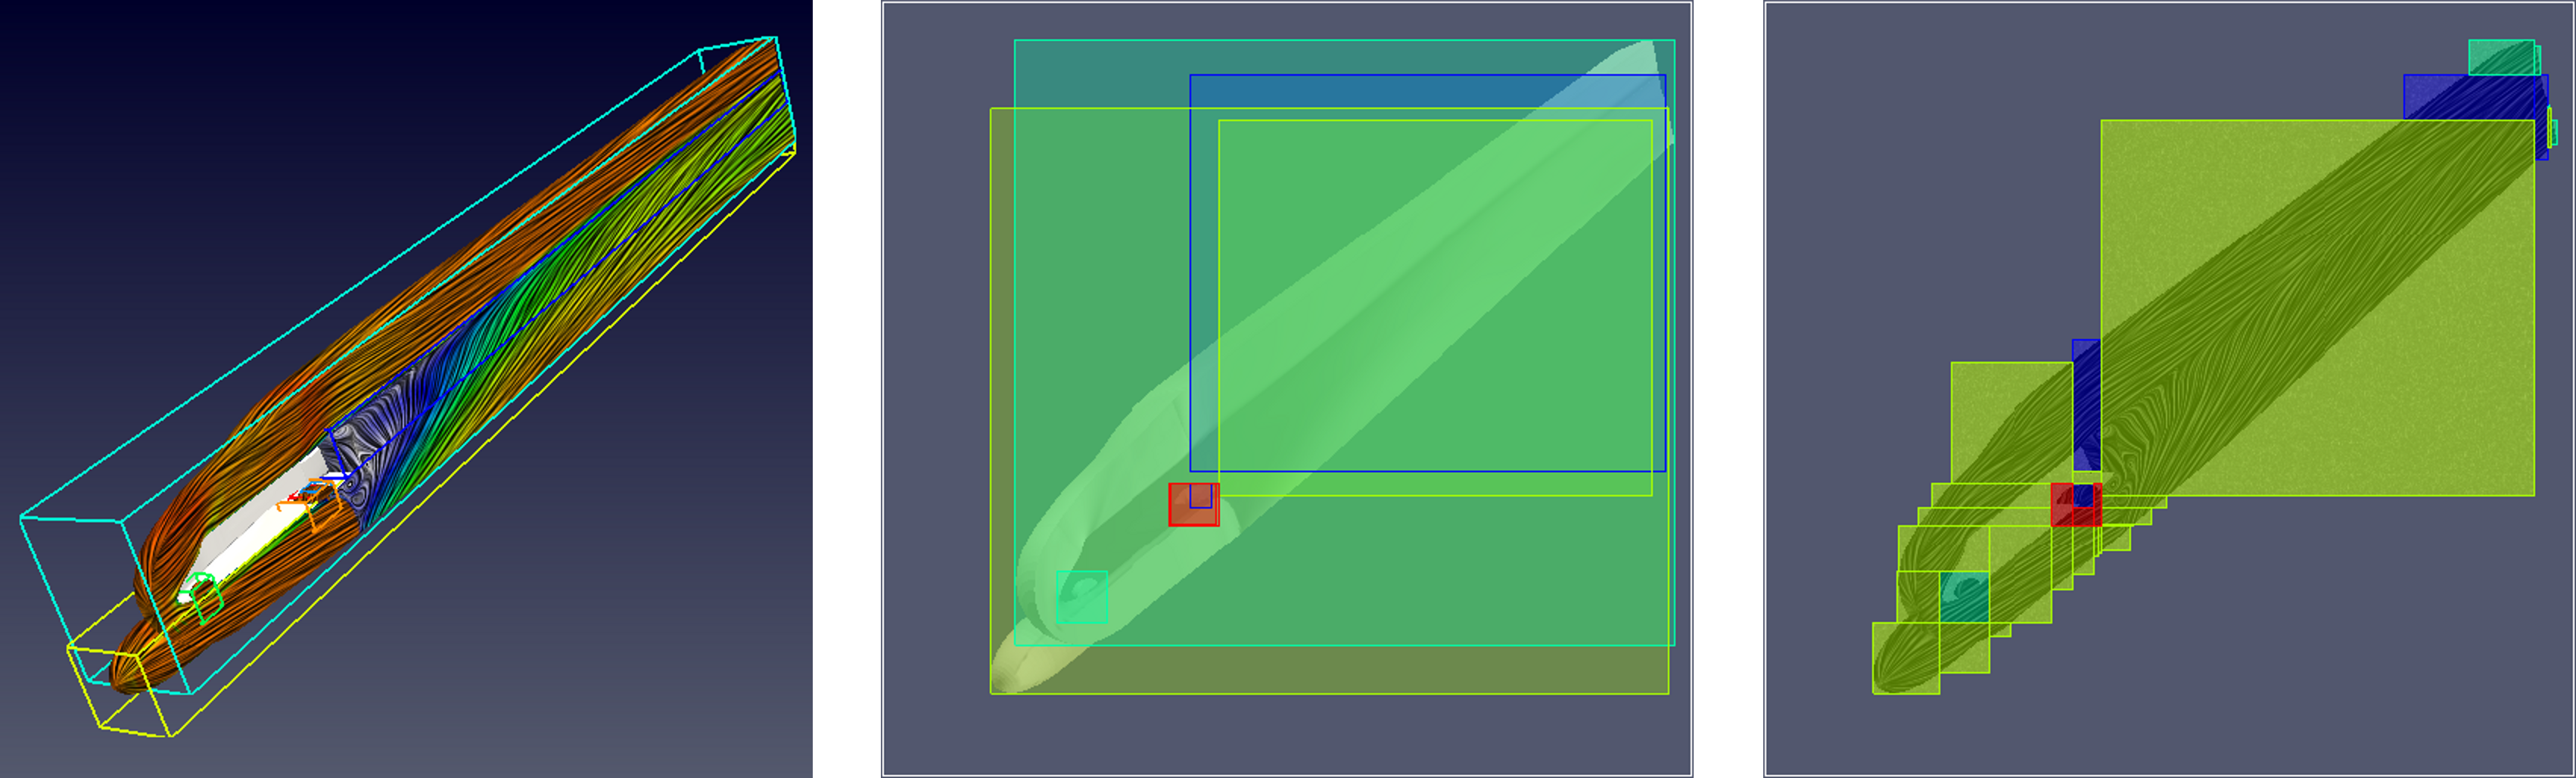
\includegraphics[width=4.75in]{shuttle-inplace-disj.png}\vspace{0.1in}\\
%   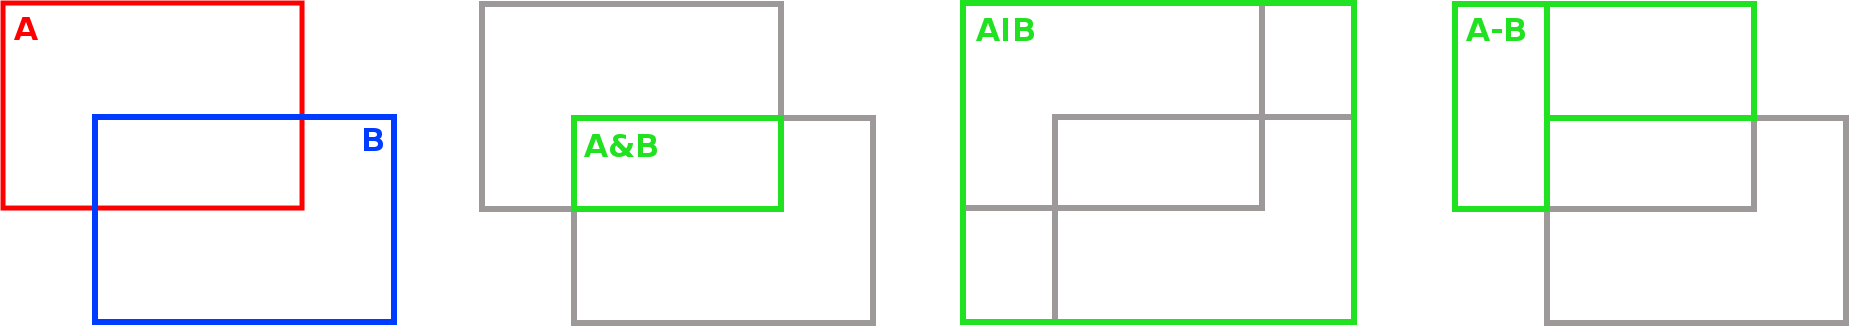
\includegraphics[width=3.25in]{operations.png}
  \end{center}
  \vspace{-0.15in}
  \begin{description}
  \item [In-place Disjoint Composite]{\it Less} lazy. Process on {\it unique parts} of existing screen space ext.
  \end{description}
  \vspace{-0.1in}
  \begin{minipage}{0.5\linewidth}
  \begin{itemize}
  \setlength{\itemindent}{-1em}
  \footnotesize 
  \item[\color{green}{\Checkmark}] reduced comminication costs by $\frac{1}{2}$ for each overlapping processor pair
  \item[\color{green}{\Checkmark}] computing once per pixel is a big win, esp. w/o GPUs
  \item[\color{green}{\Checkmark}] smaller regions further reduce comm and compute costs
  \end{itemize}
  \end{minipage}
  \begin{minipage}{0.5\linewidth}
  \only<2>{
  \begin{itemize}
  \setlength{\itemindent}{-1em}
  \footnotesize 
  \item[\color{red}{\XSolidBrush}] disjointification adds some overhead
  \item[\color{red}{\XSolidBrush}] more patches means more guardpixels means more communication
  \item[\color{red}{\XSolidBrush}] doesn't solve load balancing issues
  \end{itemize}
  }
  \end{minipage}
  \end{beamerboxesrounded}
\end{frame}

%==============================================================================
\begin{frame}{Parallelization}
    \begin{beamerboxesrounded}{Single node performance}
    \begin{minipage}{\linewidth}
    \vspace{0pt}
    \begin{center}
    \raisebox{-0.5\height}{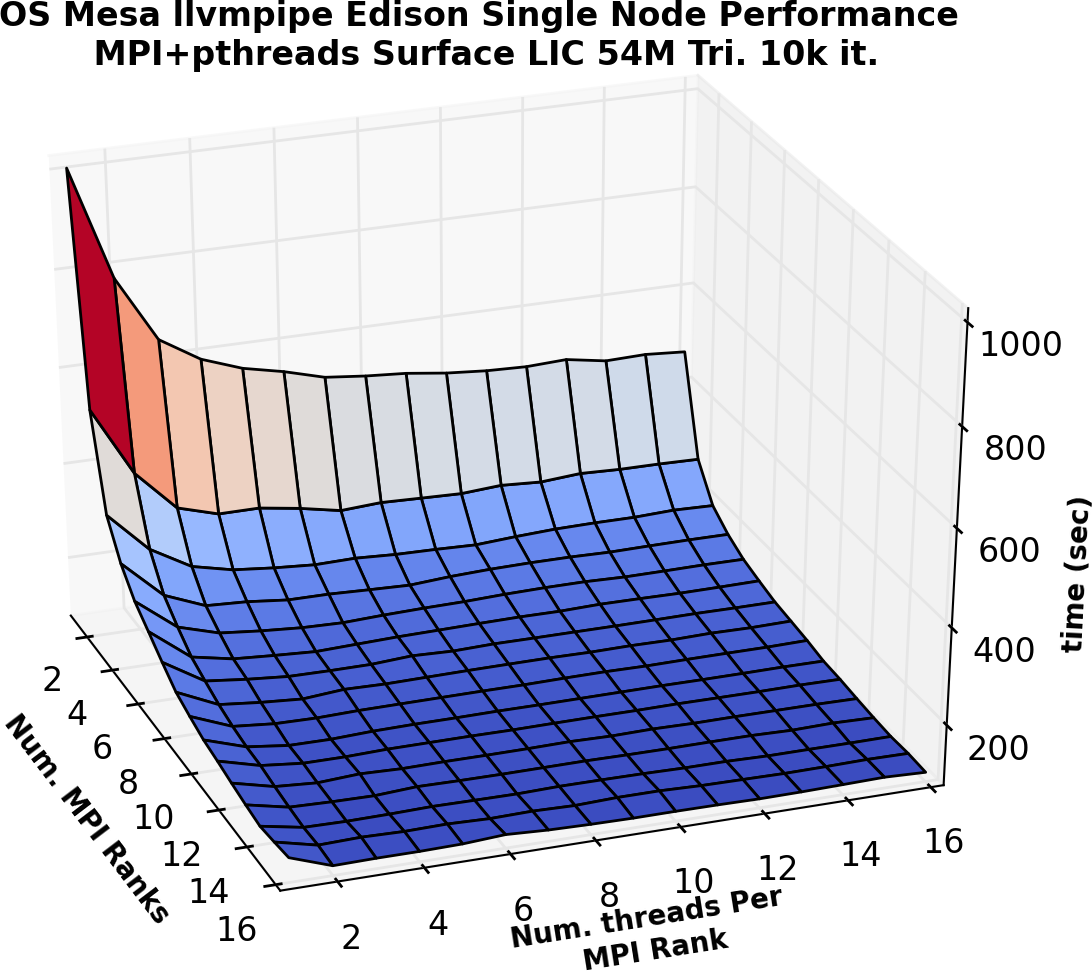
\includegraphics[width=1.4in]{llvmpipe-edison-1node.png}}\hspace{0.05in}
    \raisebox{-0.5\height}{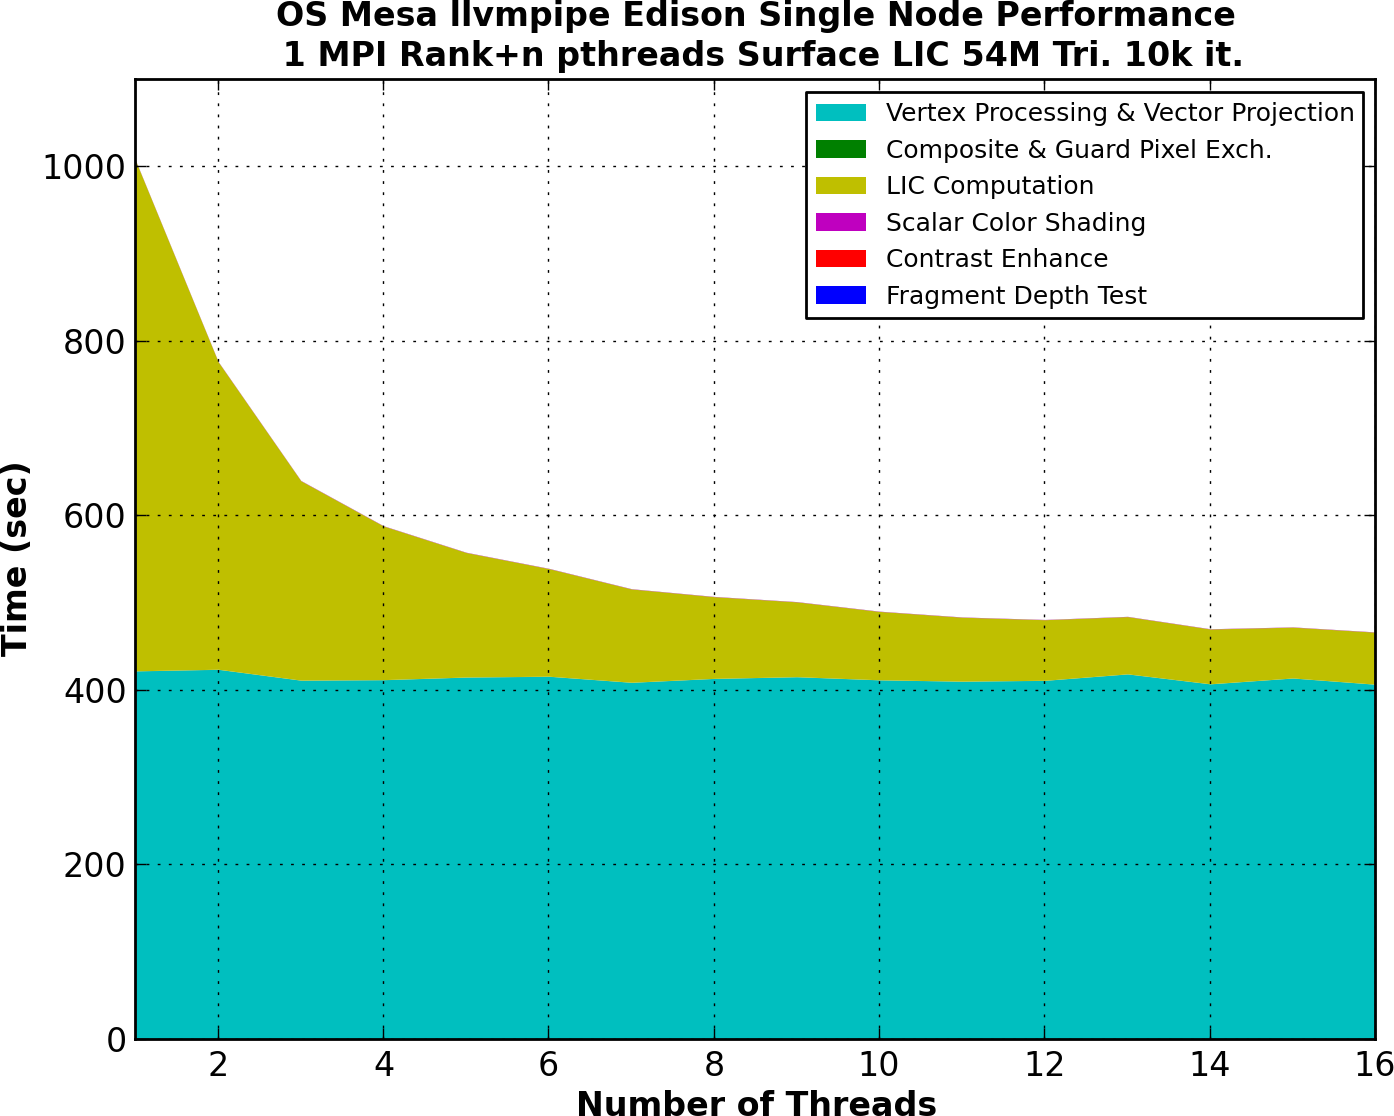
\includegraphics[width=1.4in]{llvmpipe-edison-1node-1rank-threads.png}}\hspace{0.05in}
    \raisebox{-0.5\height}{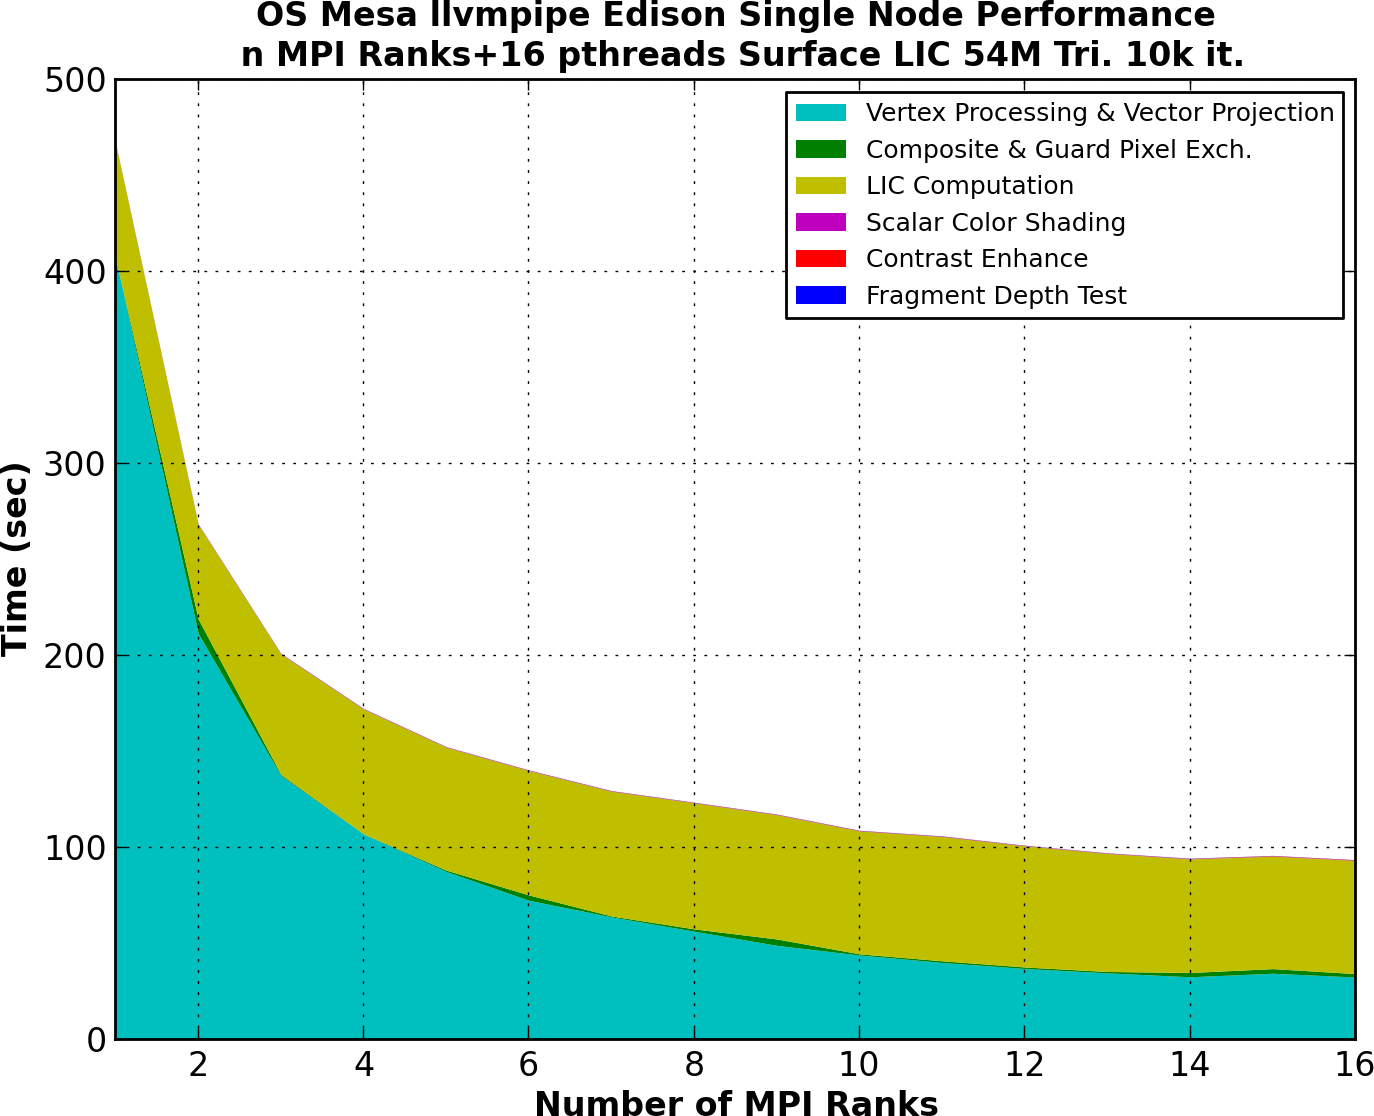
\includegraphics[width=1.4in]{llvmpipe-edison-1node-nrank-16threads.png}} 
    \end{center}
    \end{minipage}
    \vspace{-0.05in}
    \begin{itemize}
    \setlength{\itemindent}{-1em}
    \scriptsize
    \item w/o GPU
    \begin{itemize}
    \setlength{\itemindent}{-3em}
    \scriptsize
    \item Best results when number of threads on the node is equal to the number of hyperthreads.
    \item For benchmarks above and below  run 1/2 packed, 4 processes per socket, each with 4 threads.
    \end{itemize}
    \item w GPU
    \begin{itemize}
    \setlength{\itemindent}{-3em}
    \scriptsize
    \item Dual GPU nodes
    \item Run fully packed 4 processes per GPU
    \end{itemize}
    \end{itemize}
    \end{beamerboxesrounded}
\end{frame}

%==============================================================================
\begin{frame}{Parallelization}
    \vspace{-0.1in}
    \begin{beamerboxesrounded}{Performance and Scaling w/wo GPU}
    \begin{center}
    \includegraphics[width=4.60in]{lic-b-427-hr-crop.png}
    \end{center}
    \vspace{-0.1in}
    \begin{minipage}{0.45\linewidth}
    \begin{center}
    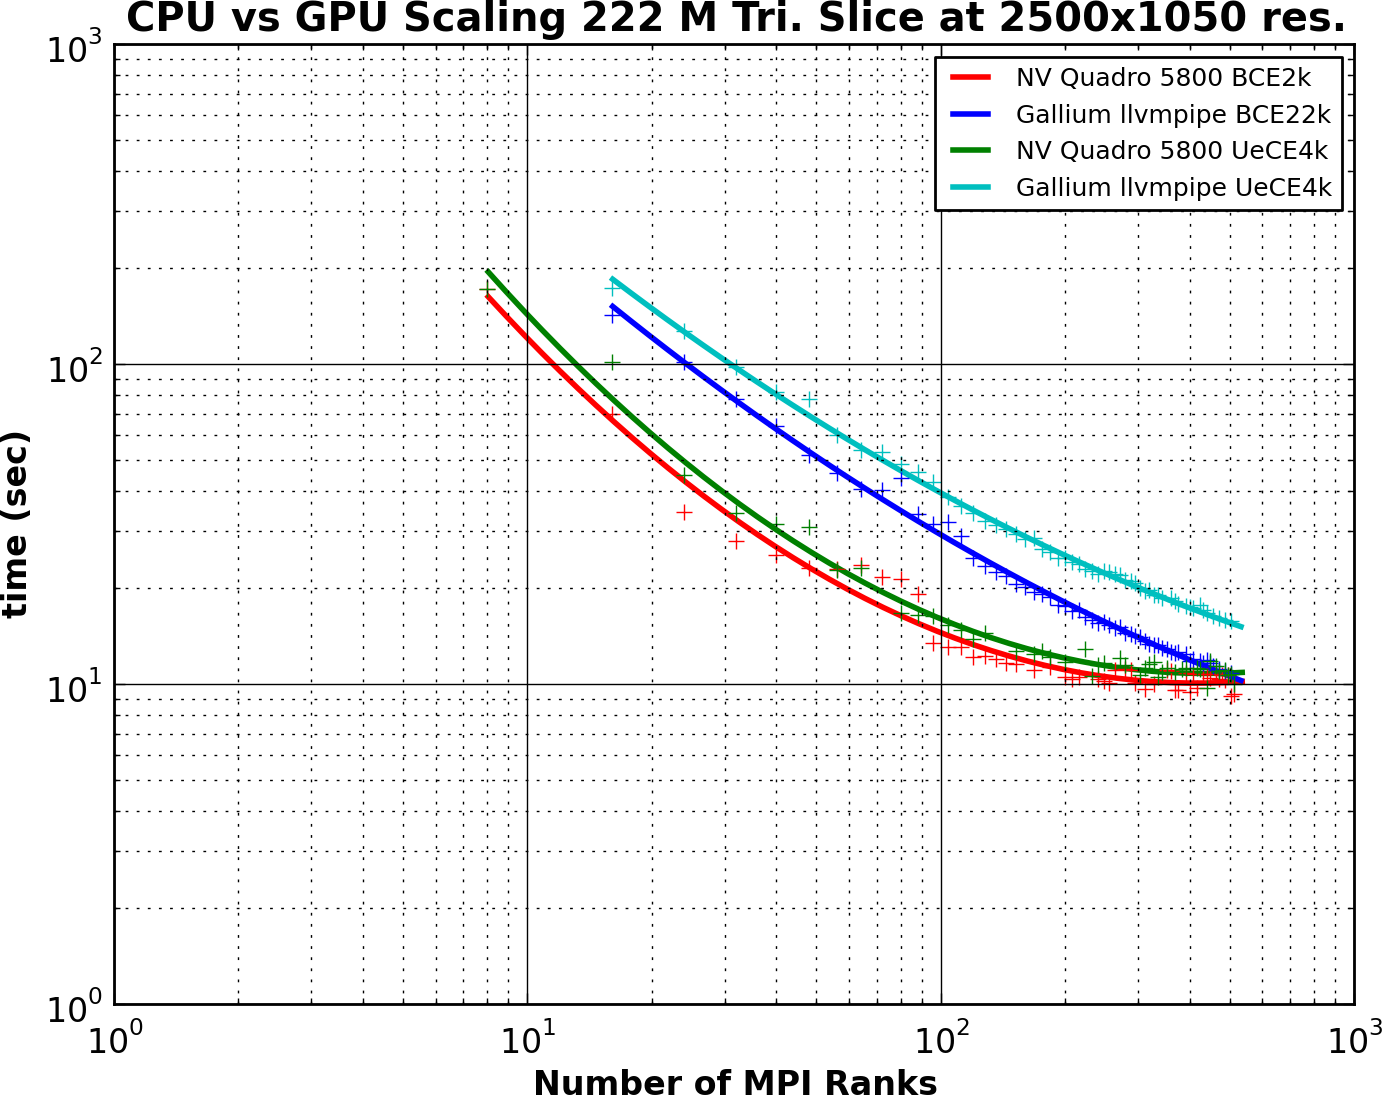
\includegraphics[width=2in]{scaling-ce-slice-gpu.png}
    \end{center}
    \end{minipage}
    \begin{minipage}{0.45\linewidth}
    \begin{itemize}
     \setlength{\itemindent}{-1em}
     \scriptsize
     \item 2D 16384x1890 cell PIC plasma turbulence simulation. 7TB of data generated 40000 cores in 72 hours on Jaguar.
     \item 222 Million triangles. 2550x1050 rendering
     \item GPU faster but CPU scales better
     \begin{itemize}
     \setlength{\itemindent}{-3em}
     \scriptsize
     \item CPU is really slow!
     \item GPU needs work to amortize the data transfers over PCI
     \item more processes $\rightarrow$ more guard pixels $\rightarrow$ more comm
     \item Edison has faster lower latency network hardware
    \end{itemize}
    \end{itemize}
    \end{minipage}
    \end{beamerboxesrounded}
\end{frame}

%==============================================================================
\begin{frame}{Parallelization}
    \begin{beamerboxesrounded}{Performance and Scaling of Compositing Alg w/wo GPU}
    \begin{minipage}{0.55\linewidth}
    \includegraphics[width=2.5in]{pr1-lic.png}
    \end{minipage}
    \begin{minipage}{0.45\linewidth}
    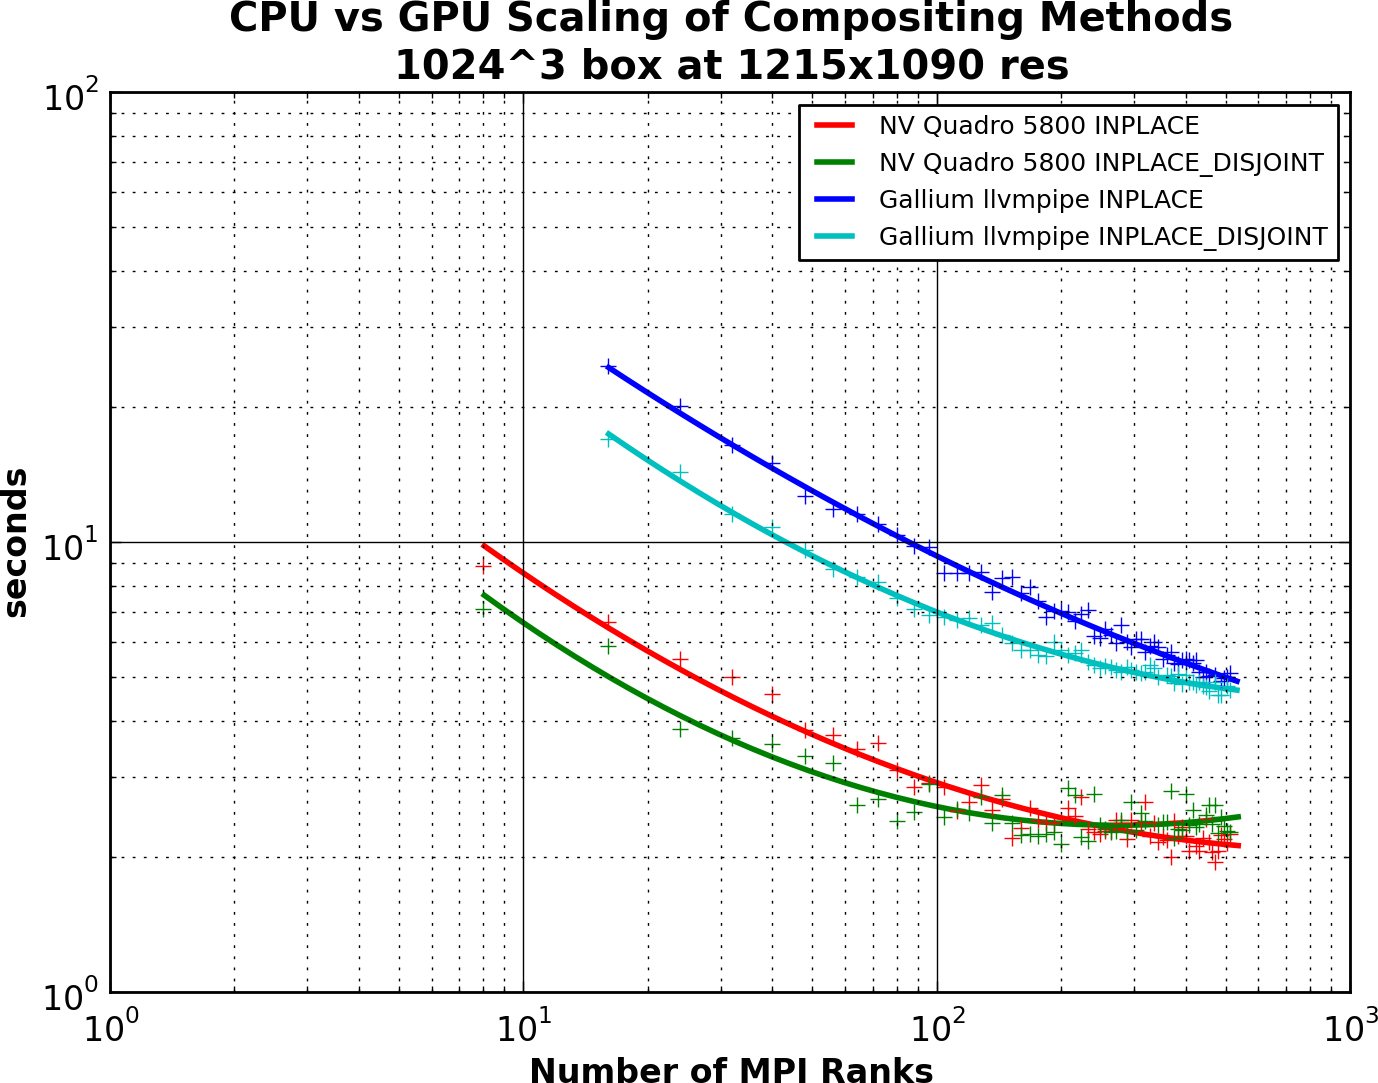
\includegraphics[width=1.8in]{scaling-composite-cube-gpu.png} \\
    \vspace{-0.1in}
    \begin{itemize}
    \setlength{\itemindent}{-1em}
    \scriptsize
    \item 3D 1024x1024 MHD plasma turbulence simulation
    \item 54 Million triangles. 1215x1090 rendering
    \item GPU faster but CPU scales better
    \begin{itemize}
    \setlength{\itemindent}{-3em}
    \scriptsize
    \item Same as before
    \item Disjointification may be resulting more guard pixels and fragmentation
    \end{itemize}
    \end{itemize}
    \end{minipage}
    \end{beamerboxesrounded}
\end{frame}

%==============================================================================
\begin{frame}{Parallelization}
    \begin{beamerboxesrounded}{Performance and Scaling of Compositing Alg w/wo GPU}
    \begin{minipage}{0.5\linewidth}
    \begin{center}
    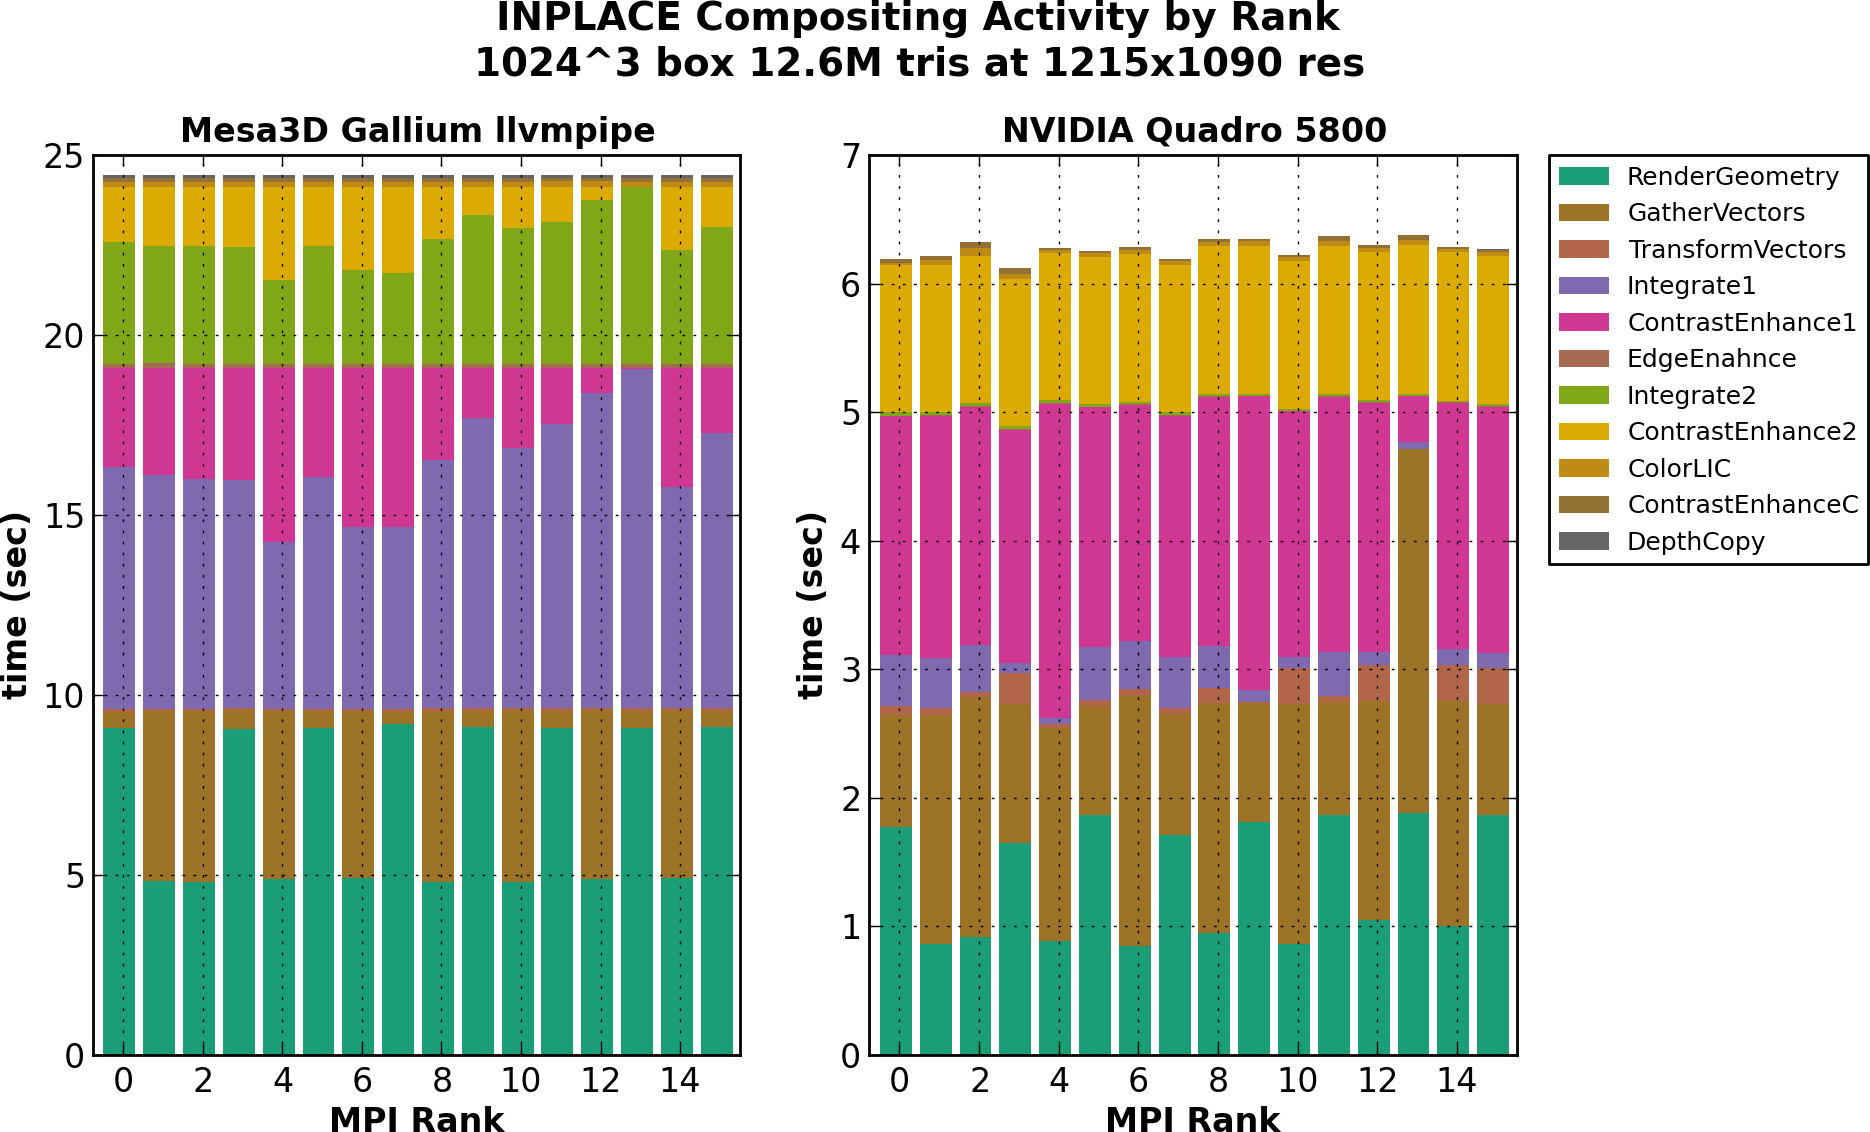
\includegraphics[width=2.25in]{scaling-gant-inplace-composite-gpu-mesa.png}\vspace{0.025in} \\
    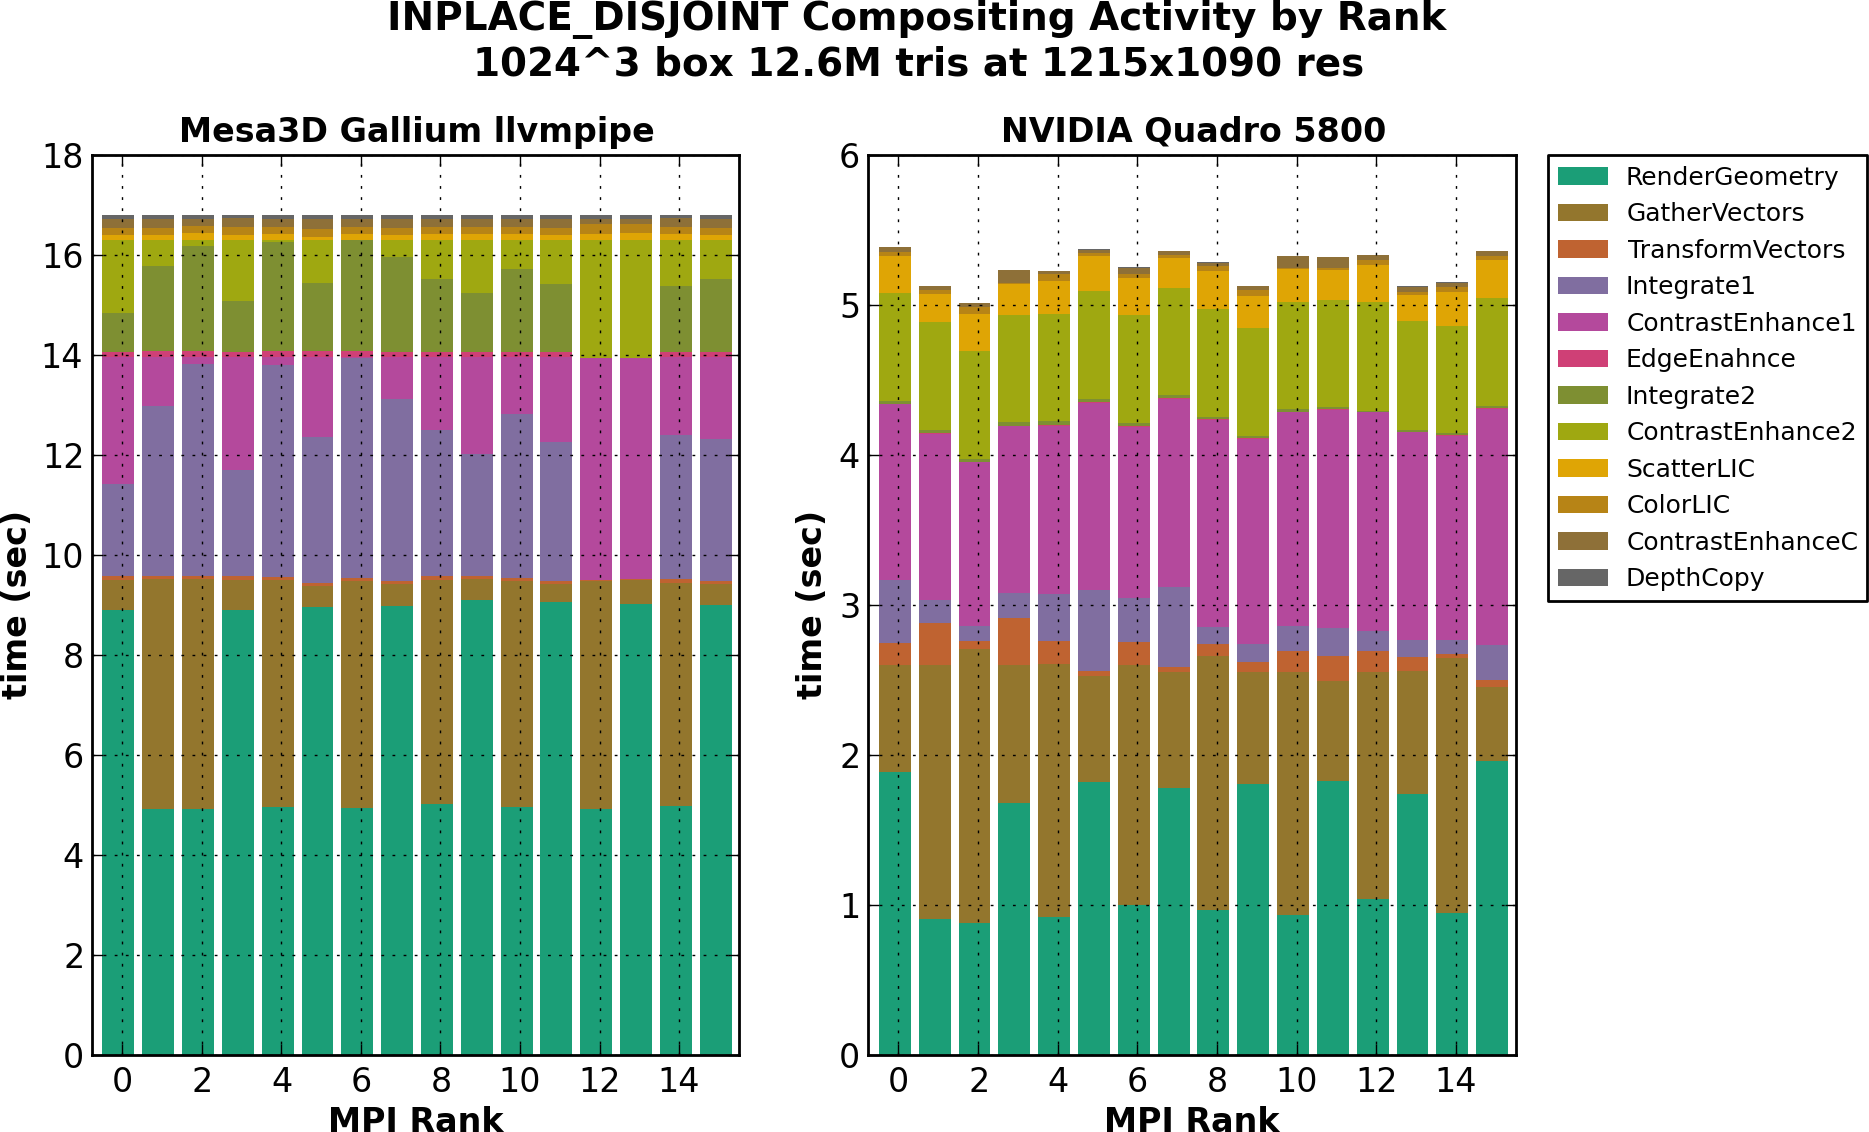
\includegraphics[width=2.25in]{scaling-gant-inplace-disjoint-composite-gpu-mesa.png}
    \end{center}
    \end{minipage}
    \begin{minipage}{0.5\linewidth}
    \begin{itemize}
    \scriptsize
%     \setlength{\itemindent}{-3em}
    \item 16 rank run, slowest run, differences are easier to spot
    \item first column : w/o GPU , disjointification shaves off time in integration (purple) and communication(brown), scatter stage(yellow second row) adding very little overhead
    \item second column : w GPU , communication is the bottleneck, gather (brown), contrast enhance (pink, yellow). 
    \end{itemize}
    \end{minipage}
    \end{beamerboxesrounded}
\end{frame}

%==============================================================================
\begin{frame}{Addressing visual and perceptual issues}
        \begin{beamerboxesrounded}{Issues addressed by our work}
        {\bf \footnotesize Motivation:}
%         \vspace{-0.1in}
        \begin{center}
        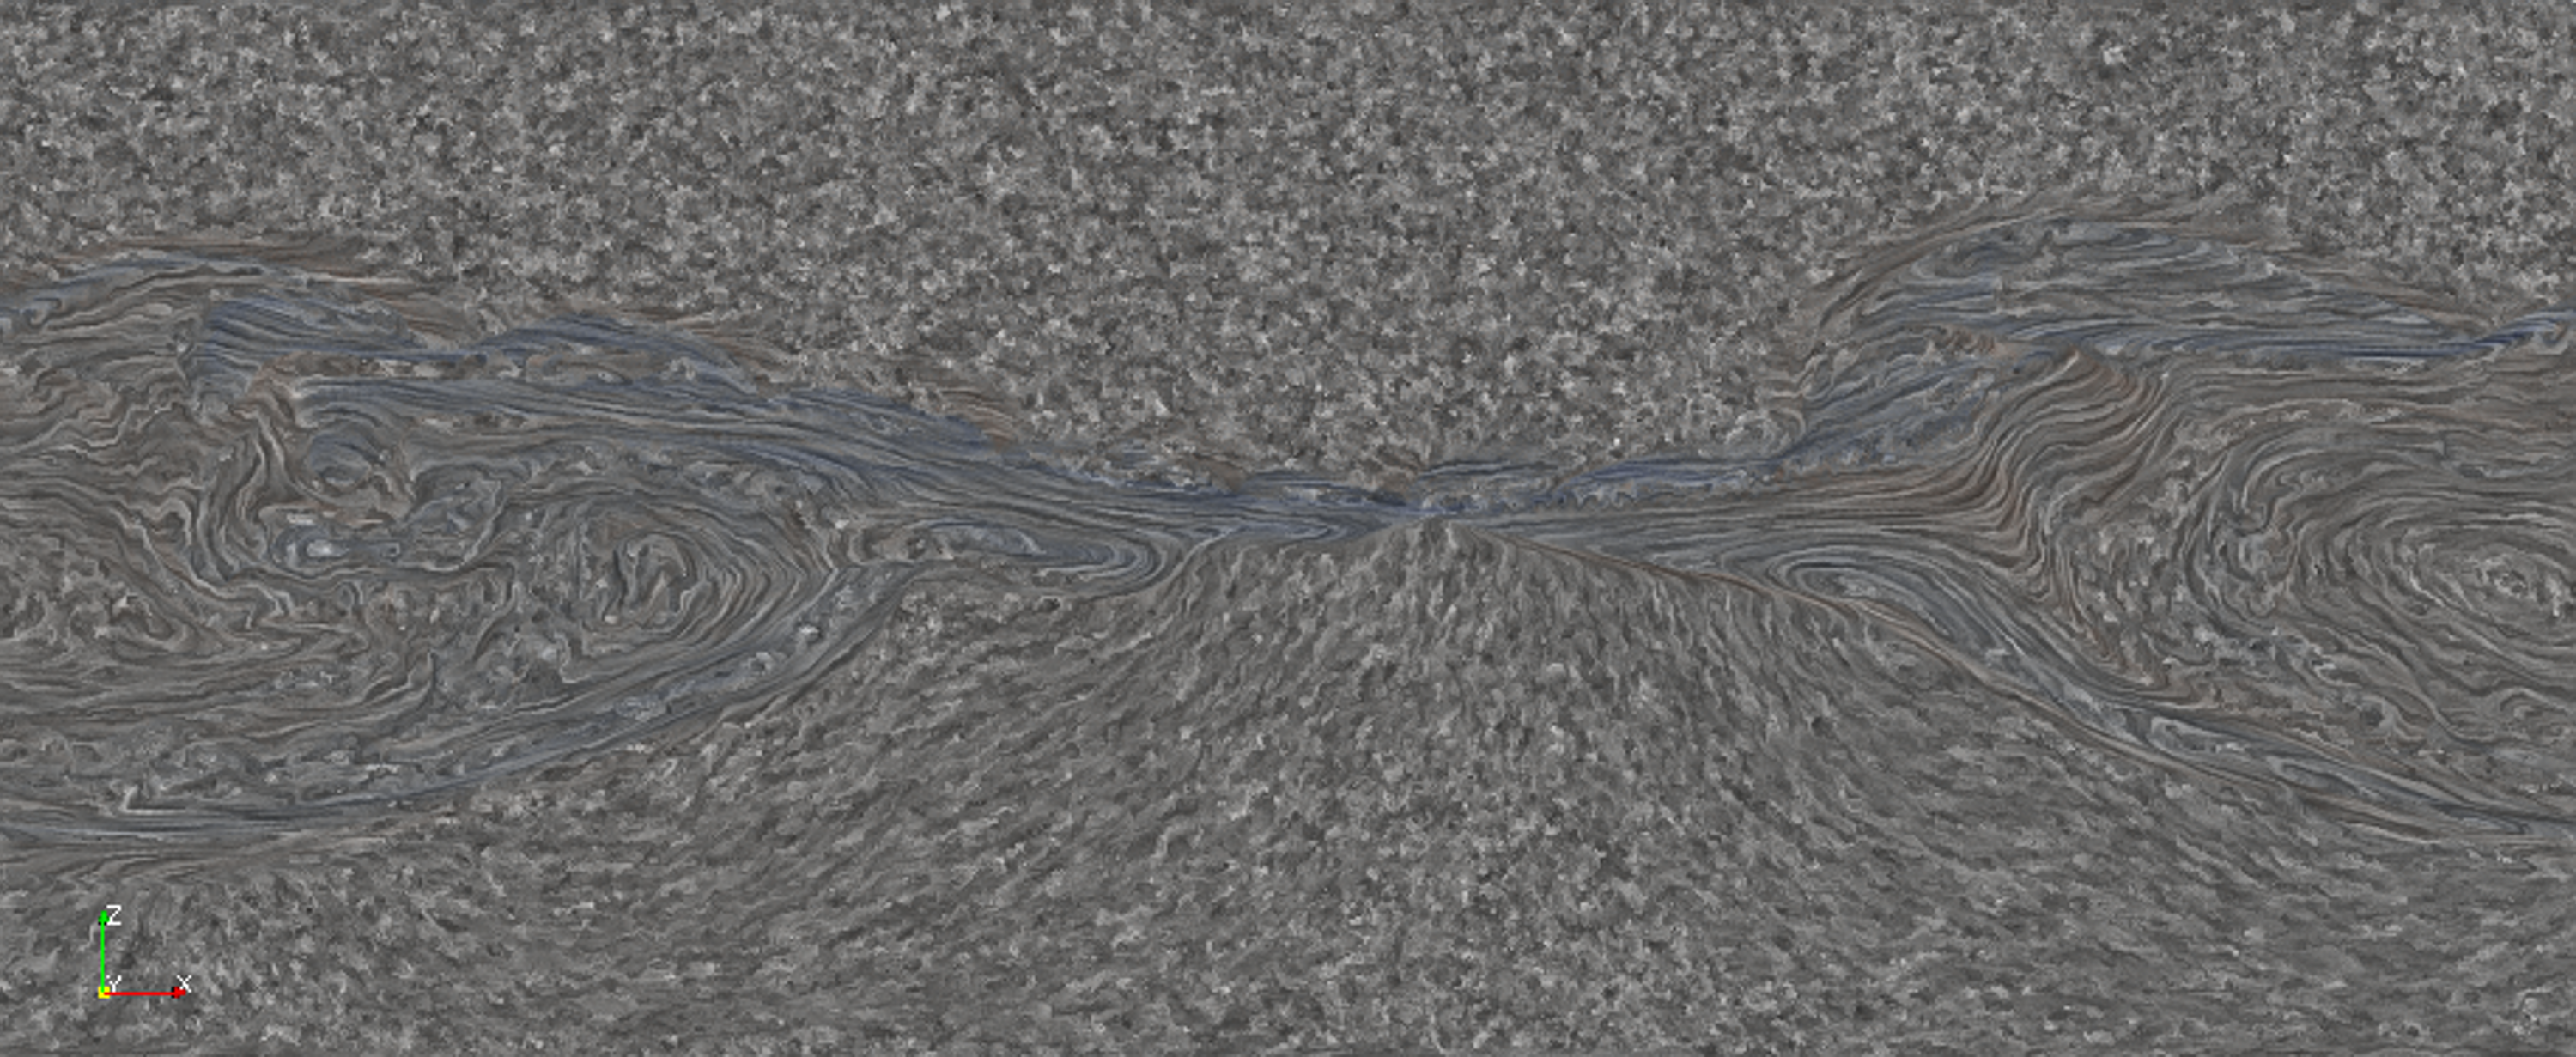
\includegraphics[width=3.65in]{motivations-vpic.png}
        \end{center}
        \vspace{-0.1in}
        {\bf Issues:}
        \begin{itemize}
        \scriptsize
        \item Results are highly dependent on inputs, many inputs, noise, vector, surface, lighting, view, camera, etc
        \item Convolution of noise naturally reduces contrast and narrows dynamic range
        \item Combination of LIC with pseudocolored lit geometry often loses subtle variations in pseducoloring, lighting.
        \end{itemize}
        {\bf  \footnotesize  What properties in LIC/shaders enable best combination with lit pseudocolored geometry?}
      \end{beamerboxesrounded}
\end{frame}

%==============================================================================
\begin{frame}{Addressing visual and perceptual issues}
    \begin{beamerboxesrounded}{First: How is LIC combined with lit pseudocolored geometry?}
    \begin{minipage}{0.5\linewidth}
    {\bf \footnotesize Blend:} \\
    \vspace{-0.1in}
    {\scriptsize
    \begin{equation}
    c_{ij} = L_{ij} * I + S_{ij} * (1 - I)
    \end{equation}
    where the indices $i,j$ identify a specific fragment, $c$ is final RGB color, $L$ is LIC gray scale value, $S$ is the scalar RGB color, and $I$ is a constant ranging from 0 to 1. } \vspace{0.1in} \\
    {\bf \footnotesize Multiply:} \\
    \vspace{-0.1in}
    {\scriptsize
    \begin{equation}
        c_{ij} = ( L_{ij} + f ) * S_{ij}
    \end{equation}
    where the indices $i,j$ identify a specific fragment, $c$ is final RGB color, $L$ is LIC gray scale intensity, $S$ is the scalar RGB color, and $f$ is a biasing parameter, typically 0, that may be used for fine tuning.} \vspace{0.1in} \\
%     \noindent {\bf Mask} \\
%     \vspace{-0.1in}
%     {\scriptsize
%     \begin{equation}
%         c_{ij} = M * I + S_{ij} * ( 1 - I )
%     \end{equation}
%     where the indices $i,j$ identify a specific fragment, $c$ is final RGB color, $M$ is the RGB mask color, $S$ is the scalar RGB color, and $I$ is the mask color intensity.} \vspace{0.1in} \\
    {\scriptsize
    \begin{equation*}
    \end{equation*}}
    \end{minipage}\hspace{0.025in}
    \begin{minipage}{0.45\linewidth}
    \begin{center}
    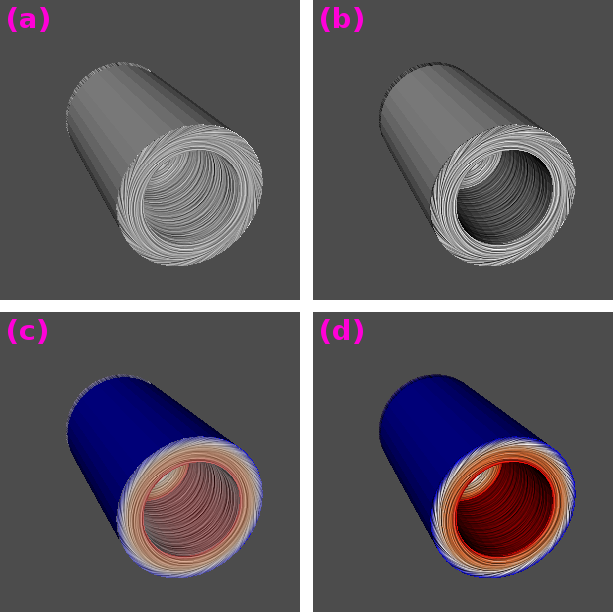
\includegraphics[width=2.25in]{blending-vs-mapping.png}
    \end{center}
    \end{minipage} \vspace{0.05in} \\
    {\bf \footnotesize Properties in LIC enable best combination with lit pseudocolored geometry:}
    \begin{itemize}
    \scriptsize
    \item LIC should have high contrast streaks with lots of pure white and black pixels.
    \item The combination process needs to preserve high contrast and dynamic range.
    \end{itemize}
    \end{beamerboxesrounded}
\end{frame}
\note{\scriptsize
{\bf blend \\}
* Decreasing $I$ to obtain brighter colors diminishes the intensity of the LIC, and vise versa.\\
* When colors are bright the LIC is difficult to see.\\
* Gives a better result curved surfaces than on planar ones.\\
{\bf multiply}\\
* Results in crisp LIC and bright colors.\\
* potentially oversaturated colors \\
}

% %==============================================================================
% \begin{frame}{Addressing visual and perceptual issues}
%   \begin{beamerboxesrounded}{Questions we tried to answer}
%   \begin{itemize}
%   \item What properties in LIC enable accurate/best combination with lit pseudocolored geometry?
%   \begin{itemize}
%   \item Highly contrasting streaks, with values close to white and black. But...
%   \end{itemize}
%   \item In convolution over long open paths streaks all approach median noise value. Can we avoid approaching a monotone result?
%   \begin{itemize}
%   \item Tune the input noise distribution. For example increase range of values in the distribution.
%   \item We're working in image space, apply techniques from image processing to correct
%   \begin{itemize}
%   \item Histogram stretching
%   \item Laplace edge enhancemnent
%   \item Anti-aliasing or smoothing soften streak transitions
%   \end{itemize}
%   \end{itemize}
%   \item Once you have the ideal LIC, what is the best way to combine with lit pseudocolored geometry? Depends...
%   \begin{itemize}
%   \item Blending, color and LIC are inversely proportional
%   \item Multiplying, LIC scales the colors
%   \end{itemize}
%   \item What can be done after the combination of colors and LIC?
%   \end{itemize}
%   \end{beamerboxesrounded}
% \end{frame}

% %==============================================================================
% \begin{frame}{SS}
% \begin{itemize}
%  \item multi-block distributed datasets where block data can overlap both on and off rank 
%  \item block overlap and hence point to point communication pattern depends on data, view, and camera 
% \end{itemize}
% \end{frame}

%==============================================================================
\begin{frame}{Addressing visual and perceptual issues}
    \vspace{-0.1in}
    \begin{beamerboxesrounded}{Noise distribution and properties}
    \begin{minipage}{0.6\linewidth}
      \begin{center}
      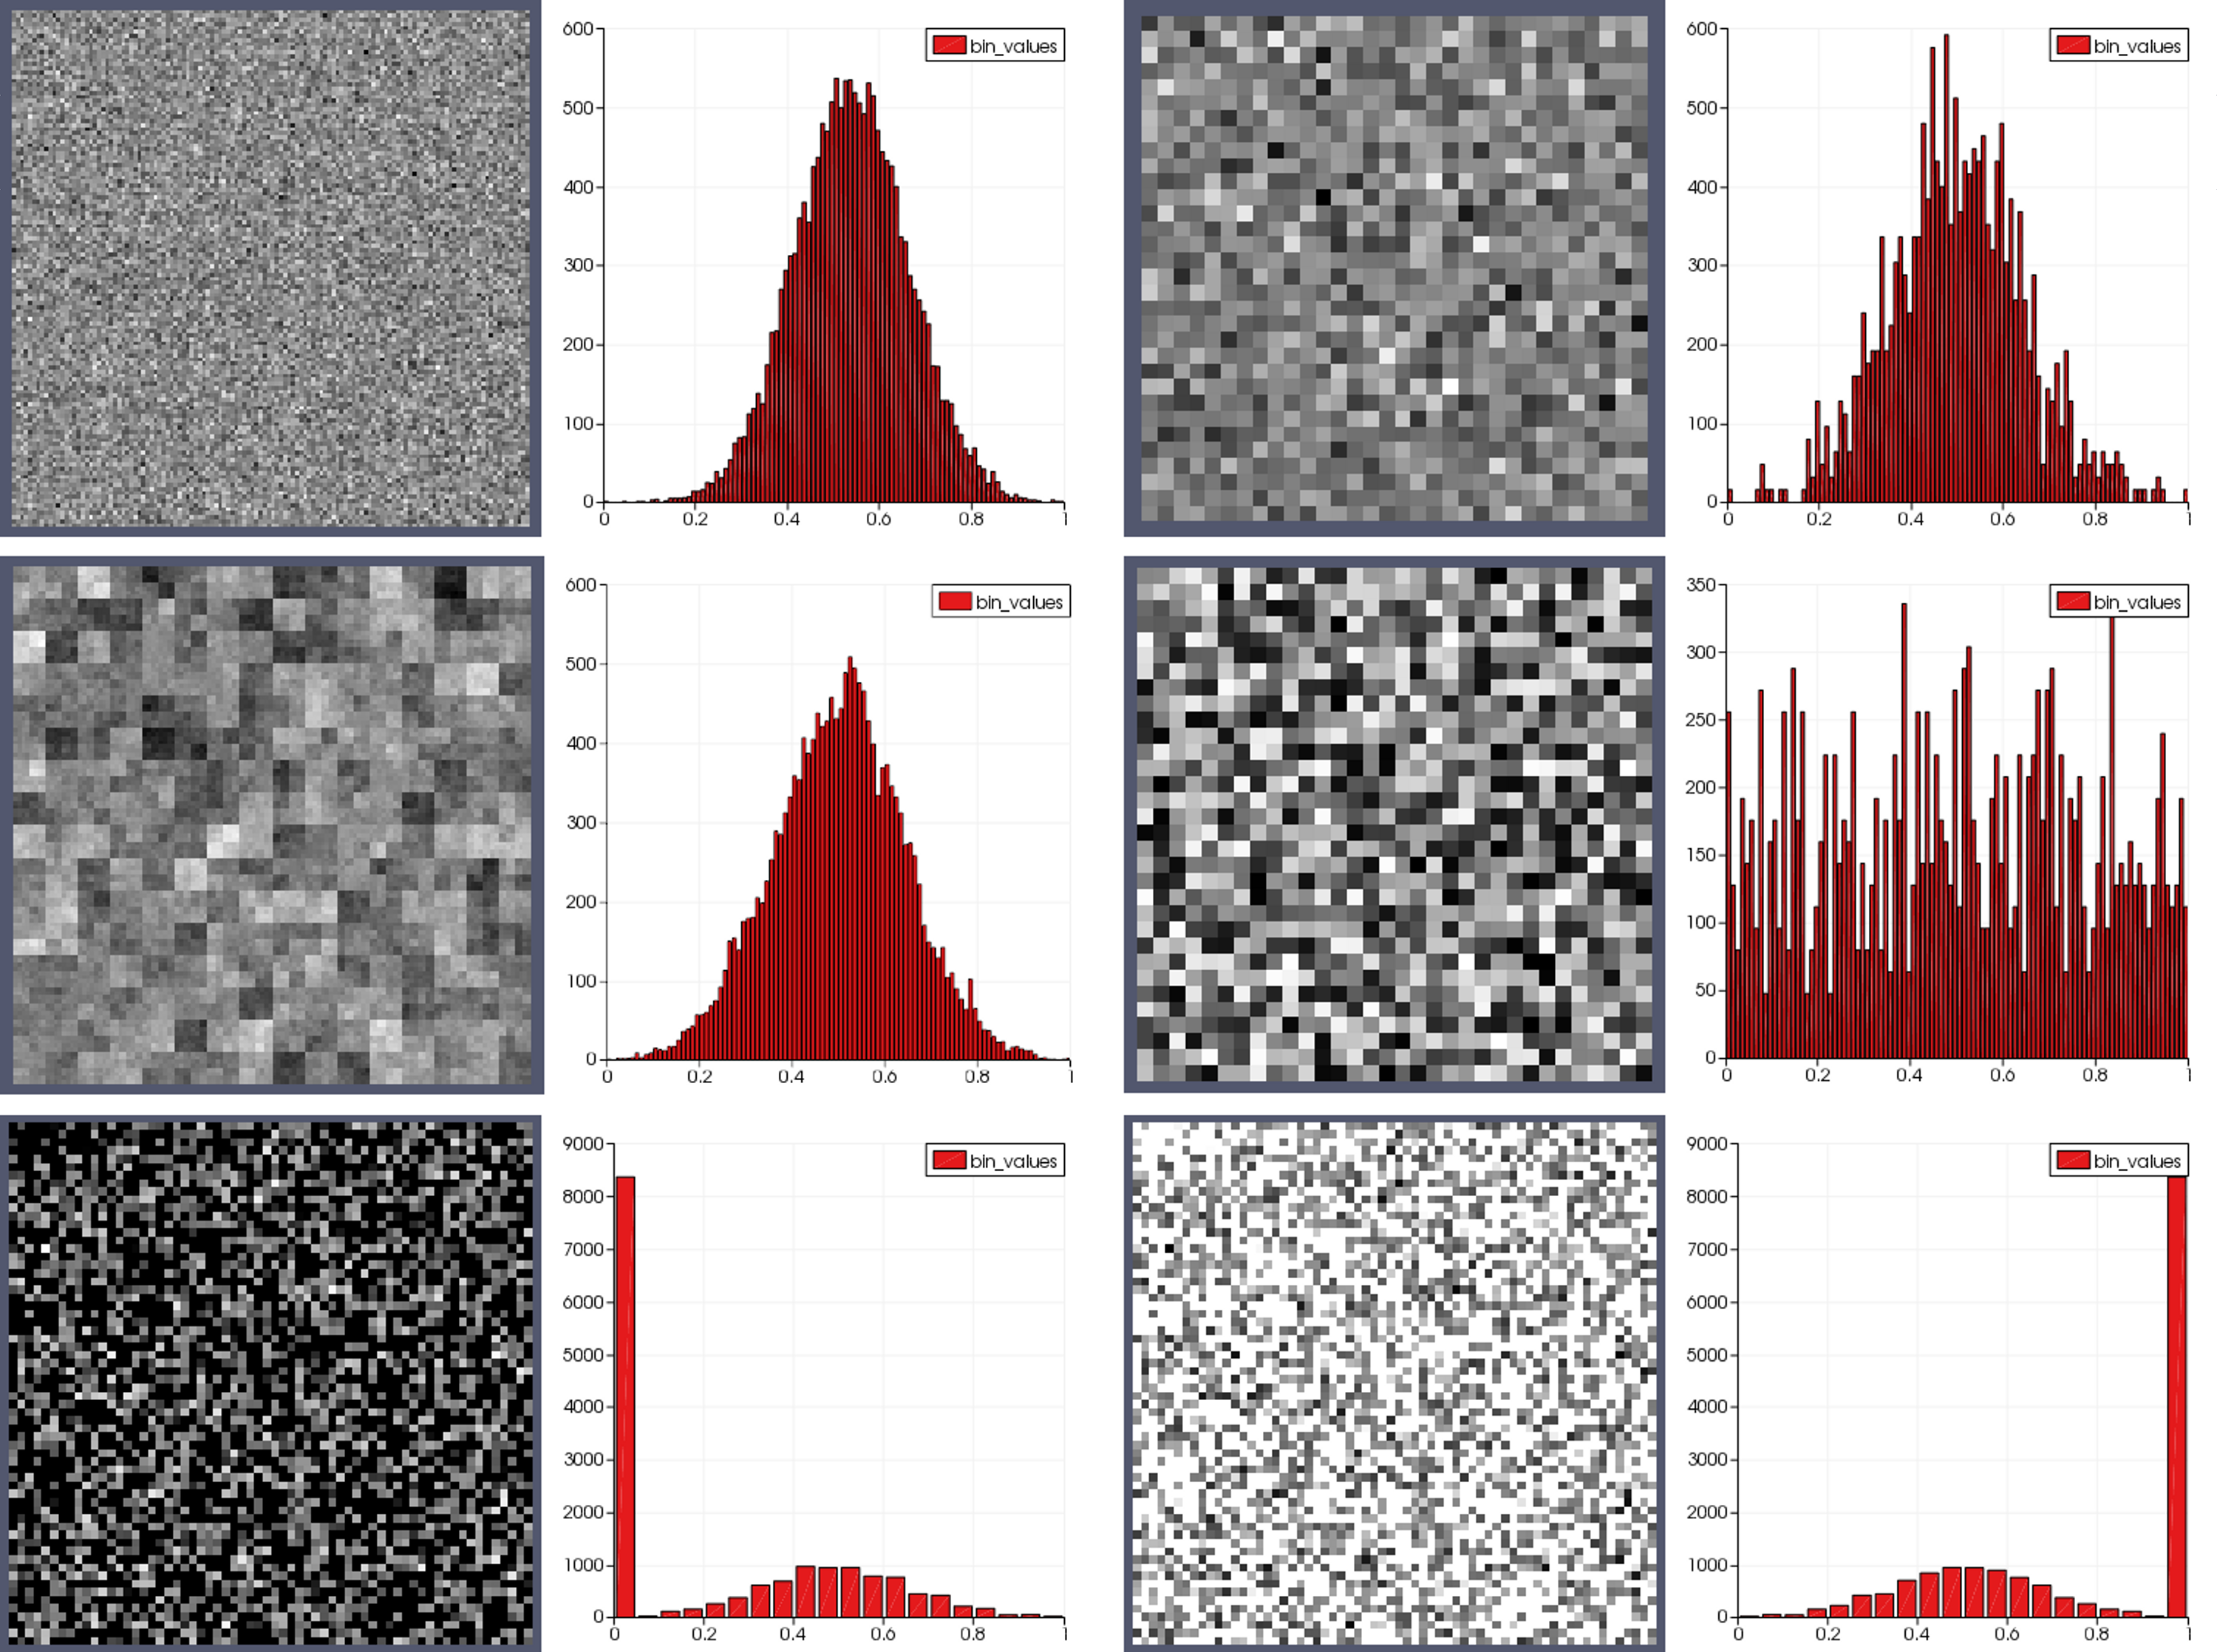
\includegraphics[width=2.45in]{noises.png}
      \end{center}
      \footnotesize
      \vspace{-0.1in}
      \begin{itemize}
        \item 9 DOF 
        \begin{itemize}
        \item size, distribution, num levels, grain size, min/max value, impulse probability, background color, seed
        \end{itemize}
        \item better control over streaking. size, width, intensity
      \end{itemize}
      \end{minipage}
    \begin{minipage}{0.35\linewidth}
       \begin{center}
       \includegraphics[width=1.85in]{ui-no-norm-gsz2-glyphs.png}\\
       \includegraphics[width=1.85in]{ui-no-norm-gsz4-glyphs-blue.png}
       \end{center}
     \end{minipage}
    \end{beamerboxesrounded}
\end{frame}

%==============================================================================
\begin{frame}{Introduction}
  \begin{beamerboxesrounded}{Screen space + OpenGL $\Rightarrow$ use image processing algorithms!}
  \begin{center}
    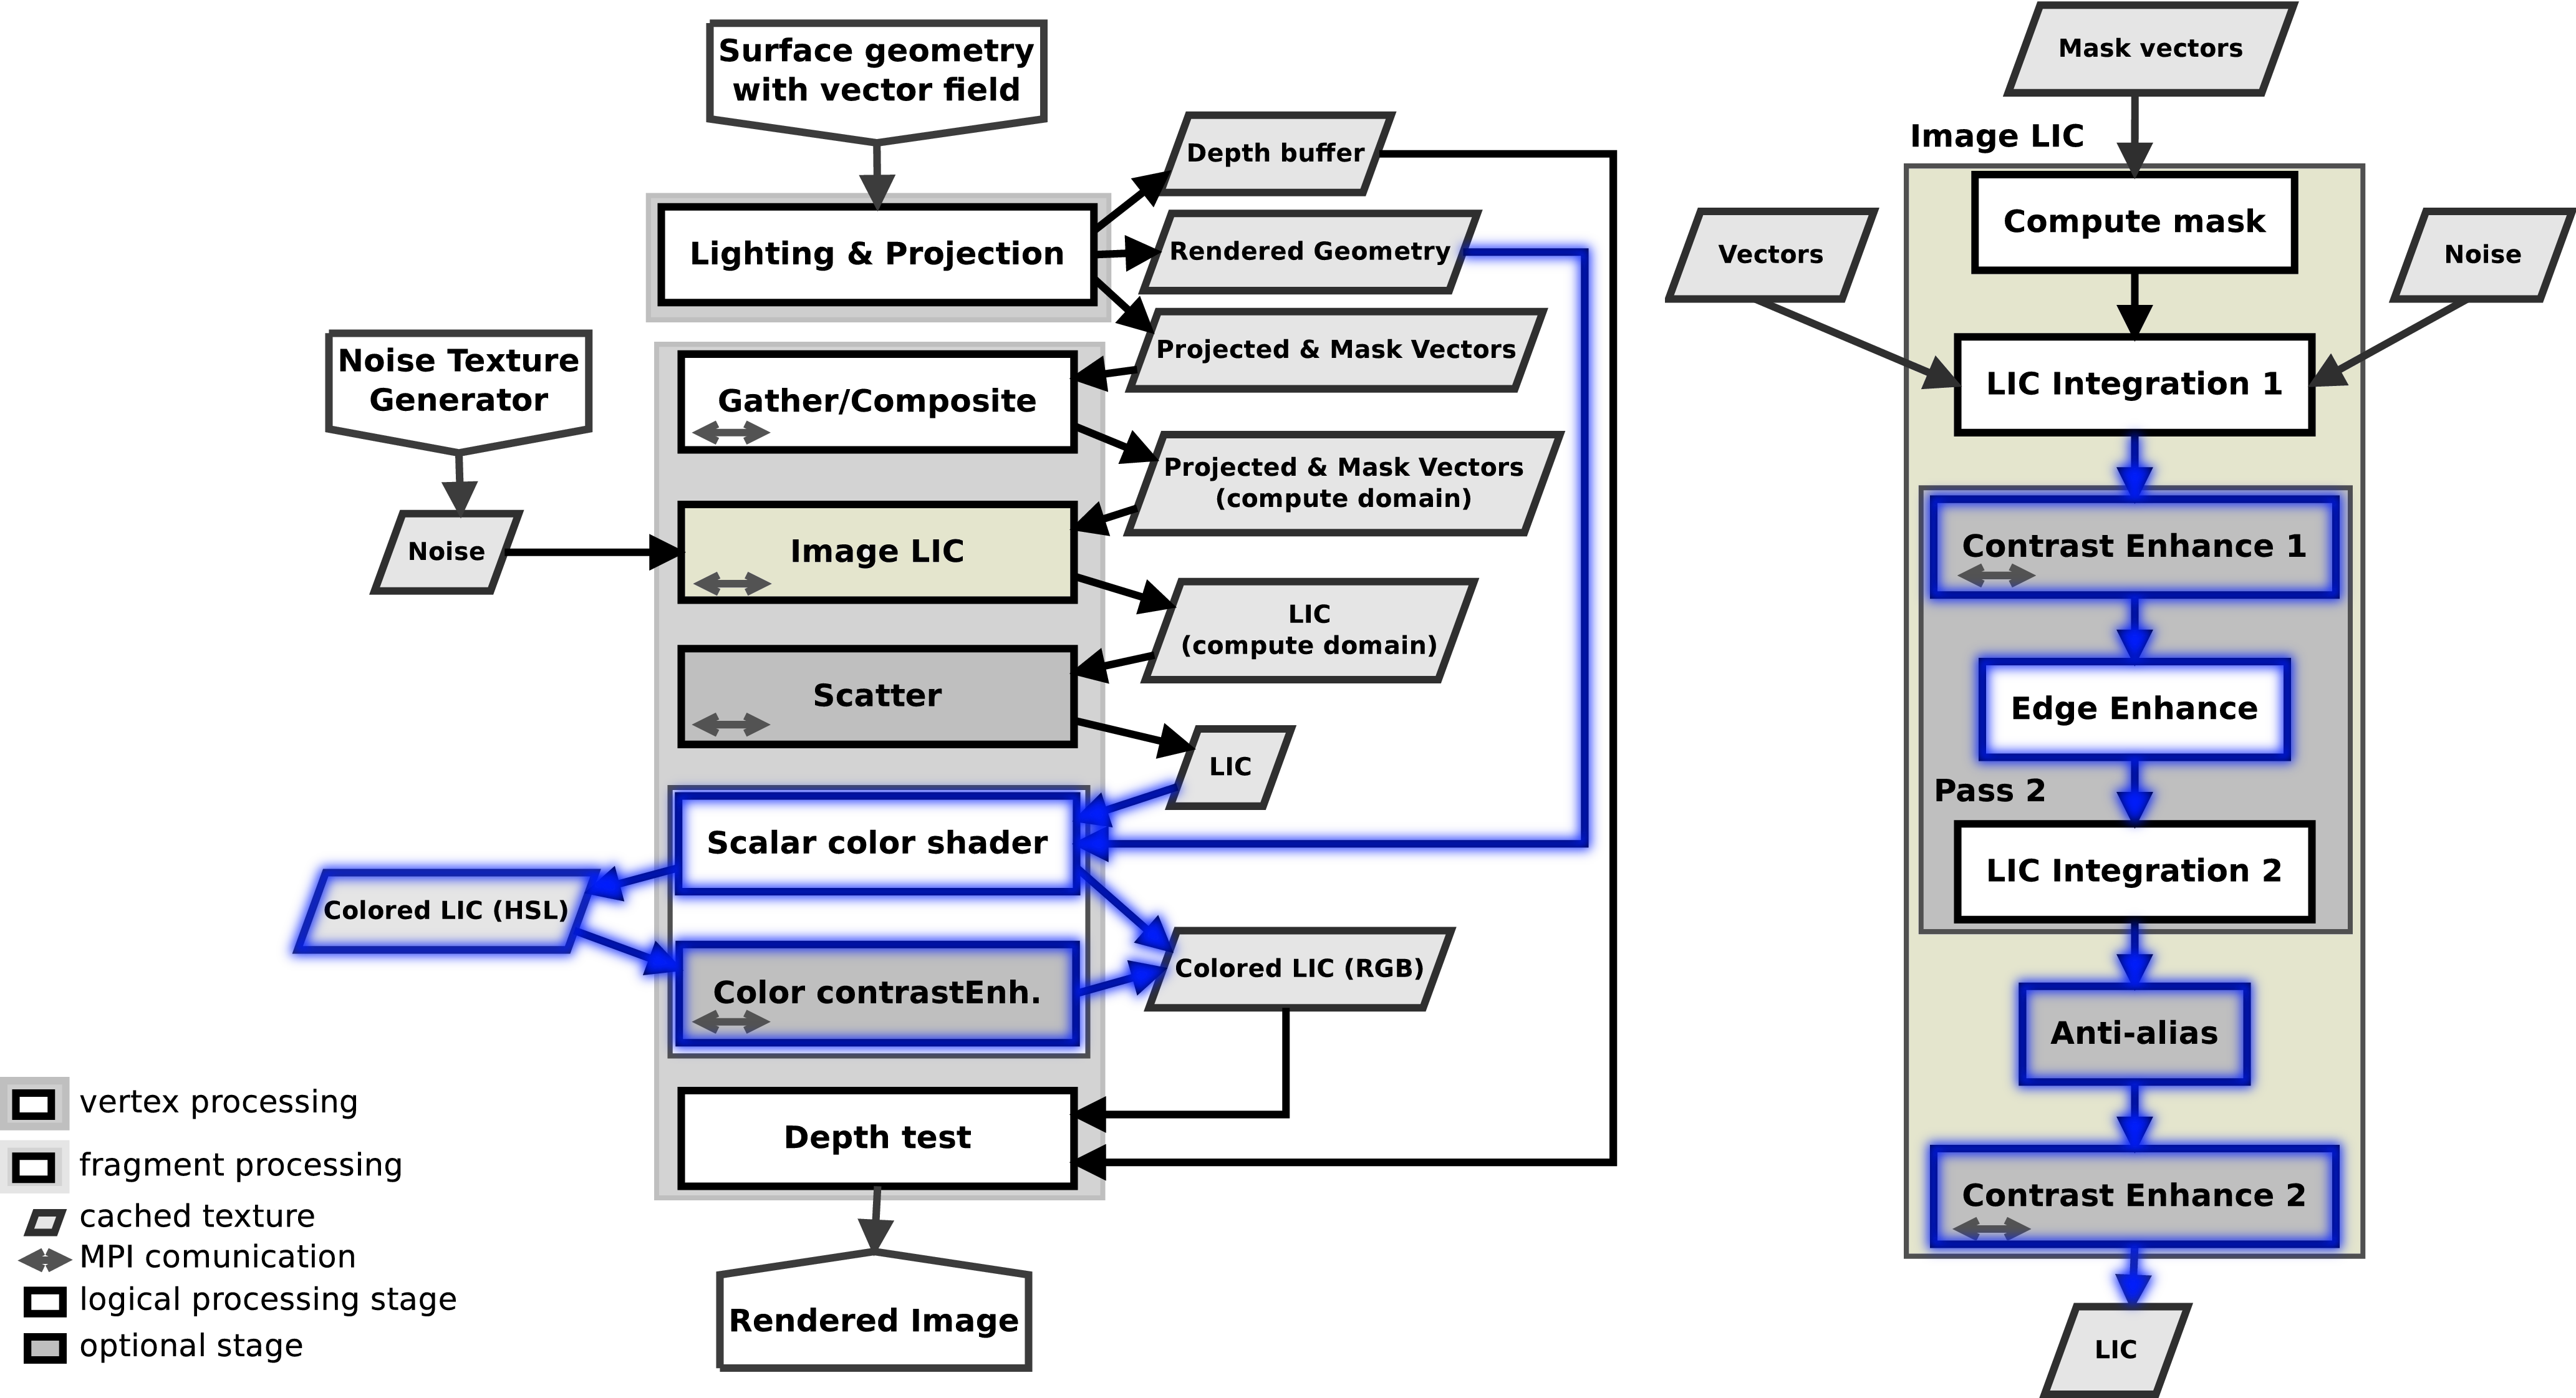
\includegraphics[width=4.2in]{ce-flow-ce.png}
  \end{center}
  \end{beamerboxesrounded}
  \end{frame}

%==============================================================================
\begin{frame}{Visual and perceptual issues}
  \begin{beamerboxesrounded}{Histogram Stretching:\\enhances streak contrast and can increase numbers of pure white and black pixels}
  \begin{center}
  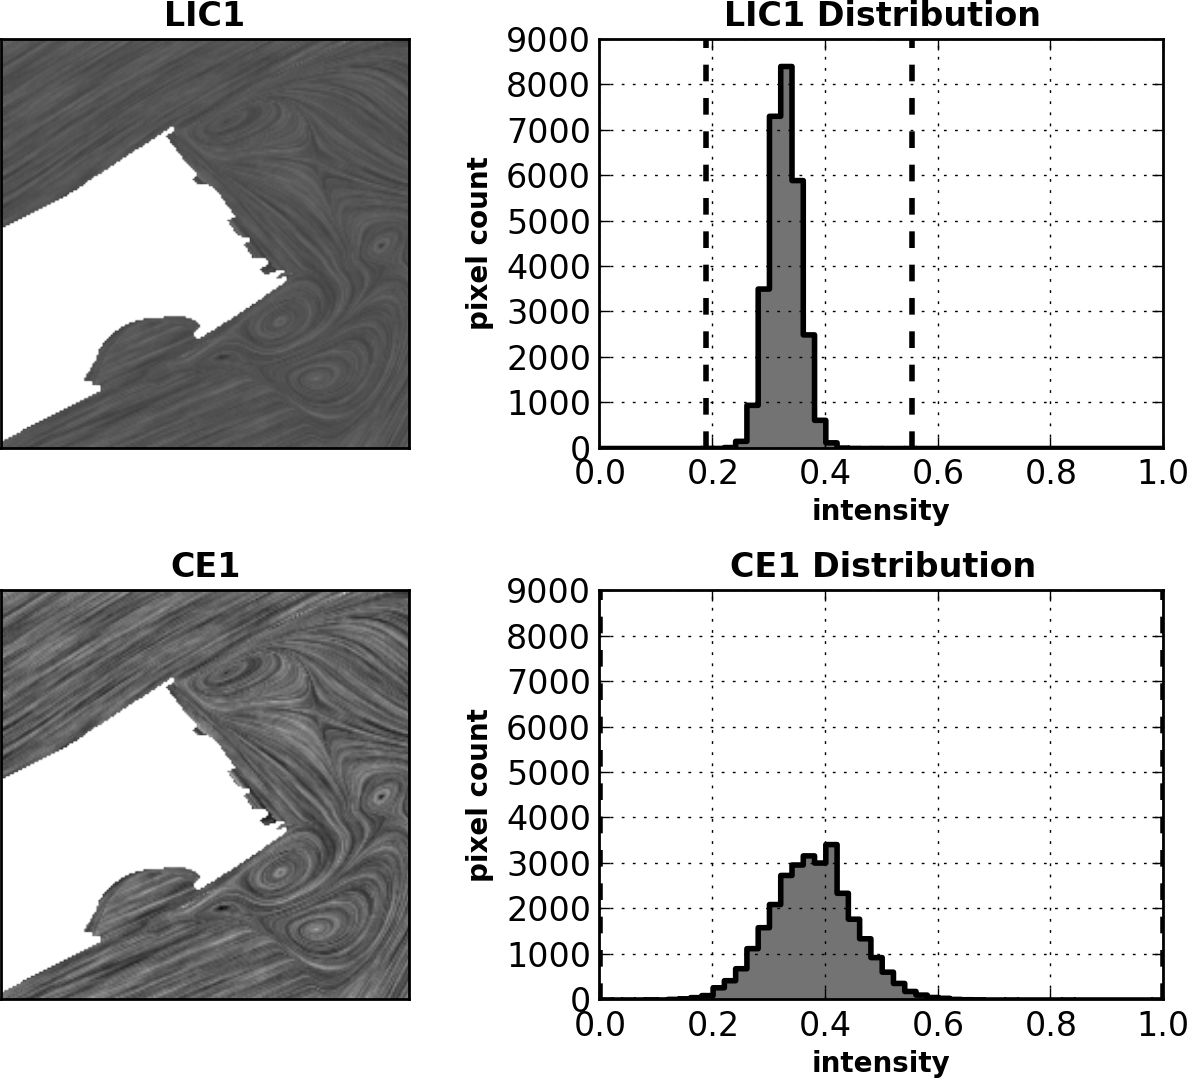
\includegraphics[width=1.6535in]{gray-ce1-curves.png}\hspace{0.0125in}
  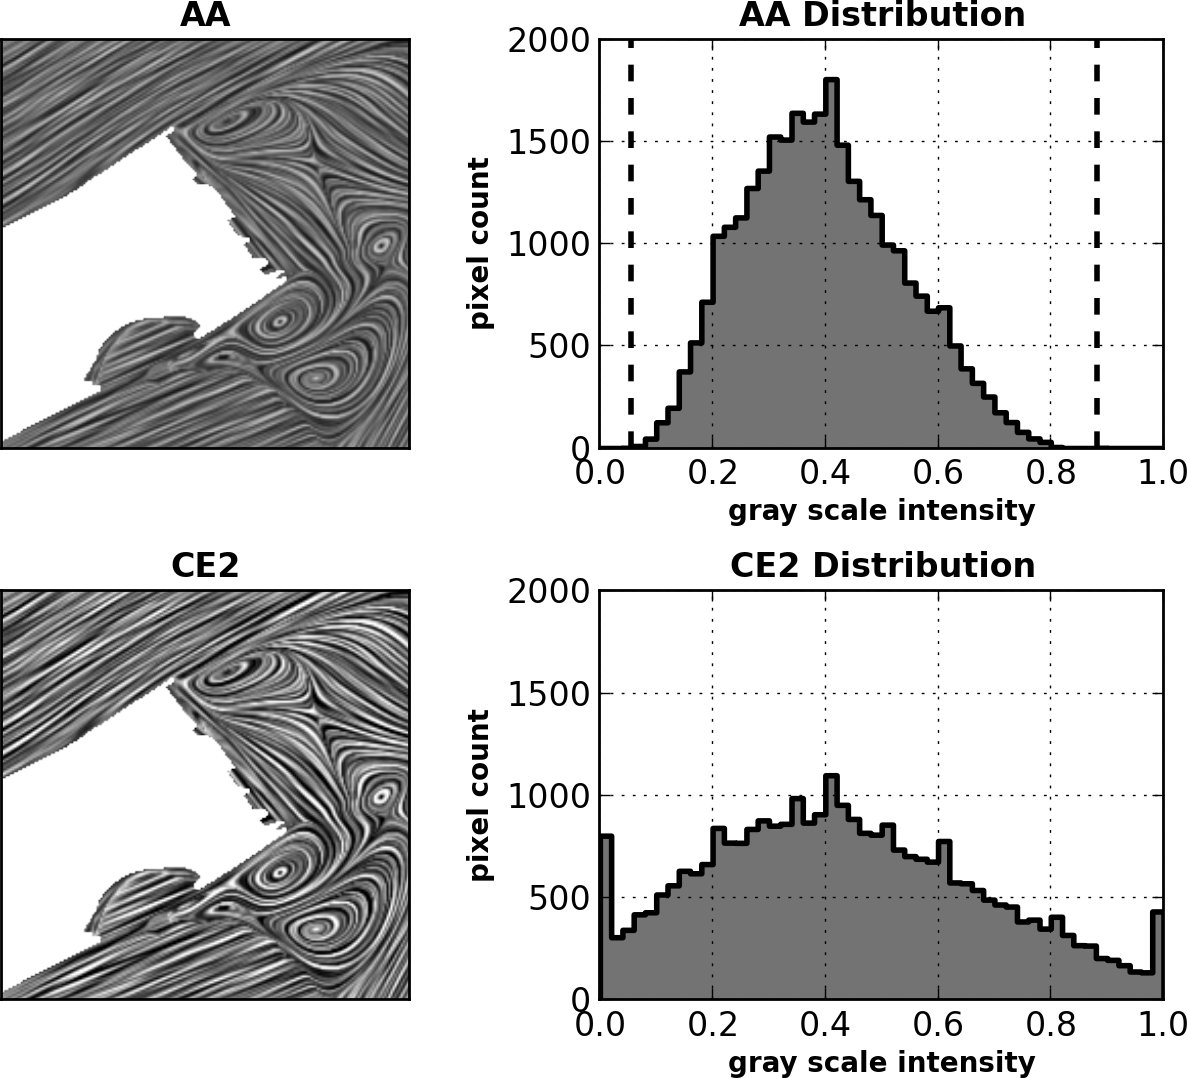
\includegraphics[width=1.6535in]{gray-ce2-curves.png}%\hspace{0.0125in}
  %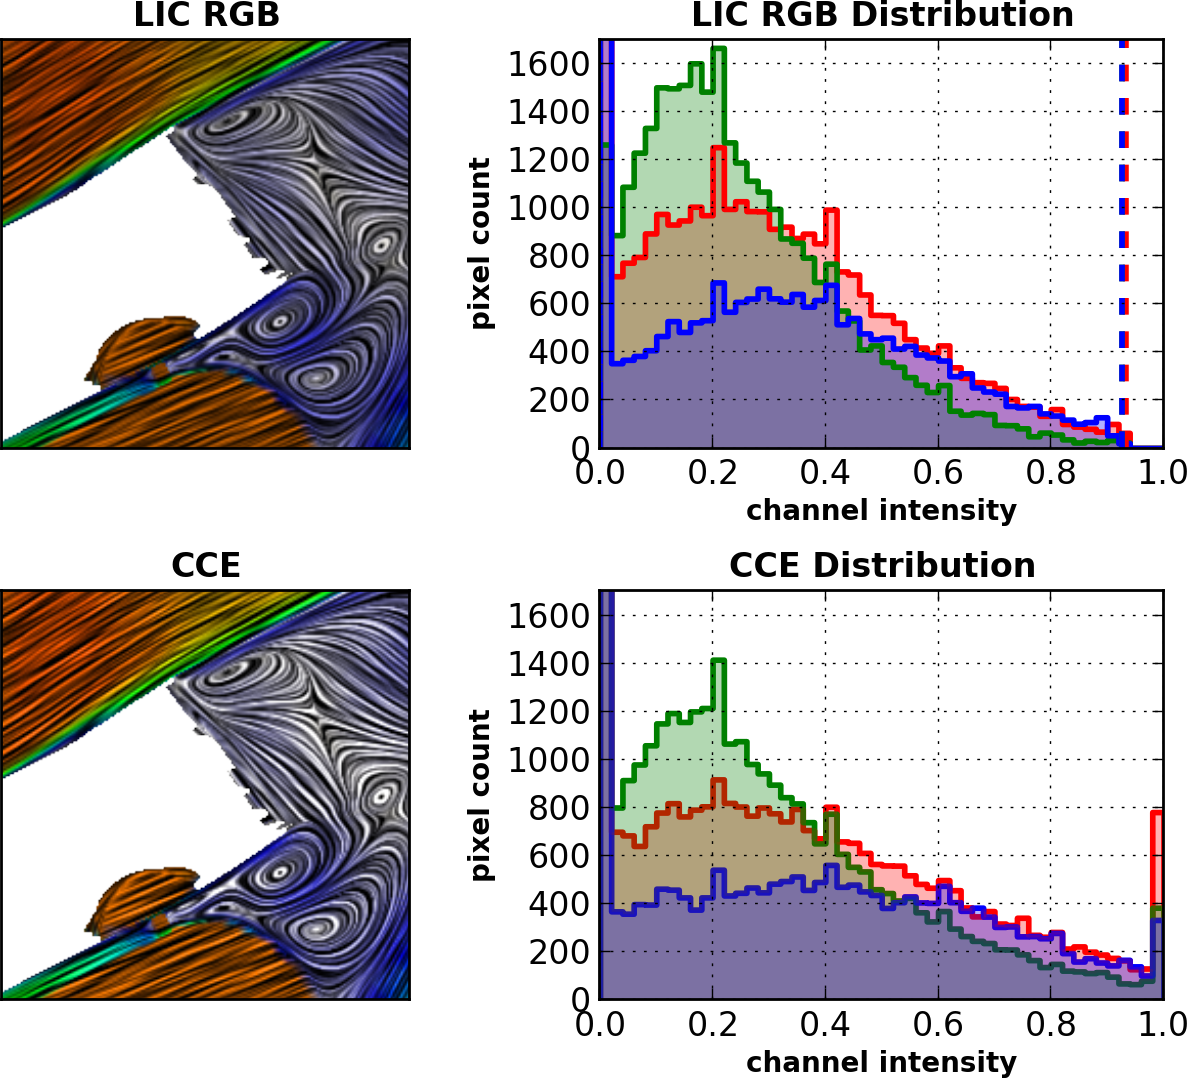
\includegraphics[width=1.535in]{color-ce-curves.png}
  \end{center}
  \vspace{-0.1in}
  {\bf \footnotesize  Linear re-mapping of intensity values}
  \scriptsize
  \begin{equation}
  I_{ij} = \frac{I_{ij} - m}{M - m}
  \end{equation}
  where, the indices $i,j$ identify a specific fragment, $I$ is the fragment's gray scale intensity, $m$ is the intensity to map to 0, $M$ is intensity to map to 1.\\
  {\bf \footnotesize Automating the procedure}
  \begin{equation}
  m = min(I) + F_{m} * ( max(I) - min(I) )
  \end{equation}
  \begin{equation}
  M = max(I) - F_{M} * ( max(I) - min(I) ) 
  \end{equation}
  where, min/max are computed on all fragments, $F_m$ and $F_M$ are optional adjustment factors.
  \end{beamerboxesrounded}
\end{frame}

%==============================================================================
\begin{frame}{Visual and perceptual issues}
    \begin{beamerboxesrounded}{Color Space Histogram Stretching:\\Applied on lightness channel after HSL conversion}
    \begin{center}
    \href{run:B-Ue-2-30fps-10fps.mp4}{\includegraphics[width=4.5in]{B-Ue-2-0333-hist.png}}\\
    \includegraphics[width=4.5in]{B-Ue-0333-hist.png}
    \end{center}
    \end{beamerboxesrounded}
\end{frame}

%==============================================================================
\begin{frame}{Interactivity}
    \begin{beamerboxesrounded}{efficienciently respond to user tweaks}
    \begin{minipage}{0.2\linewidth}
    \begin{center}
    \only<1>{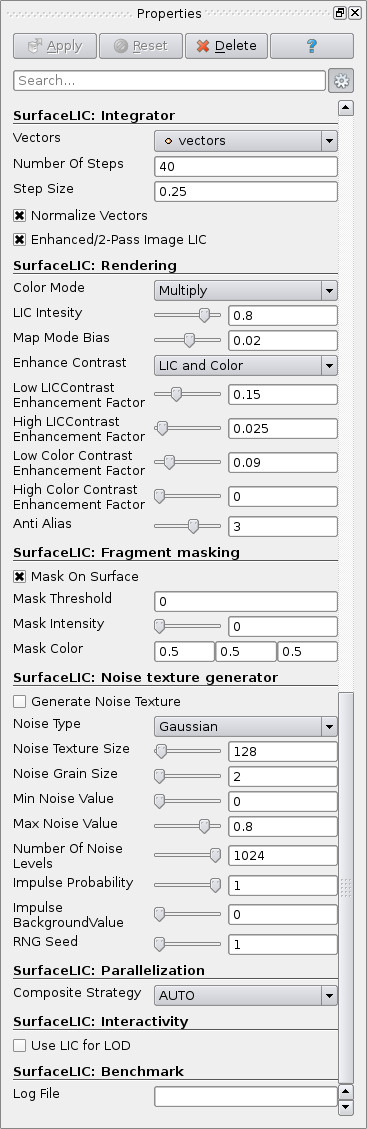
\includegraphics[width=0.9in]{pv-ui.png}}
    \only<2>{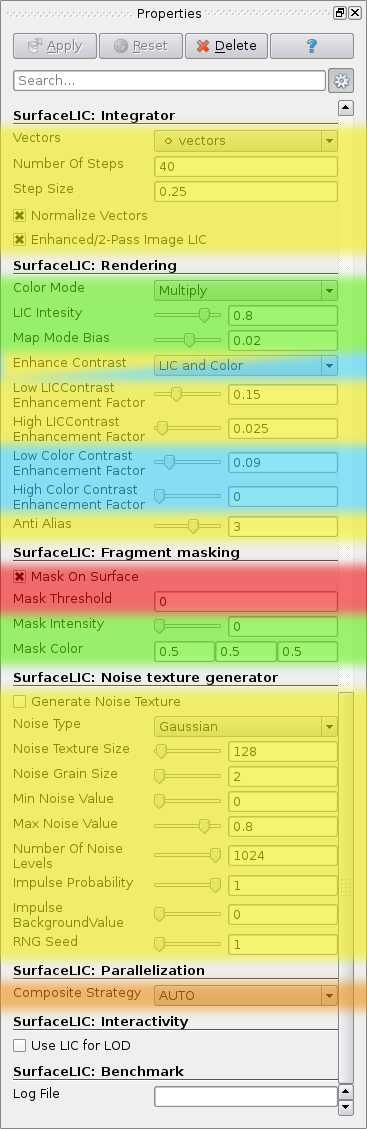
\includegraphics[width=0.9in]{pv-ui-groups.png}}
    \end{center}
    \end{minipage}
    \begin{minipage}{0.75\linewidth}
    \begin{center}
    \only<1>{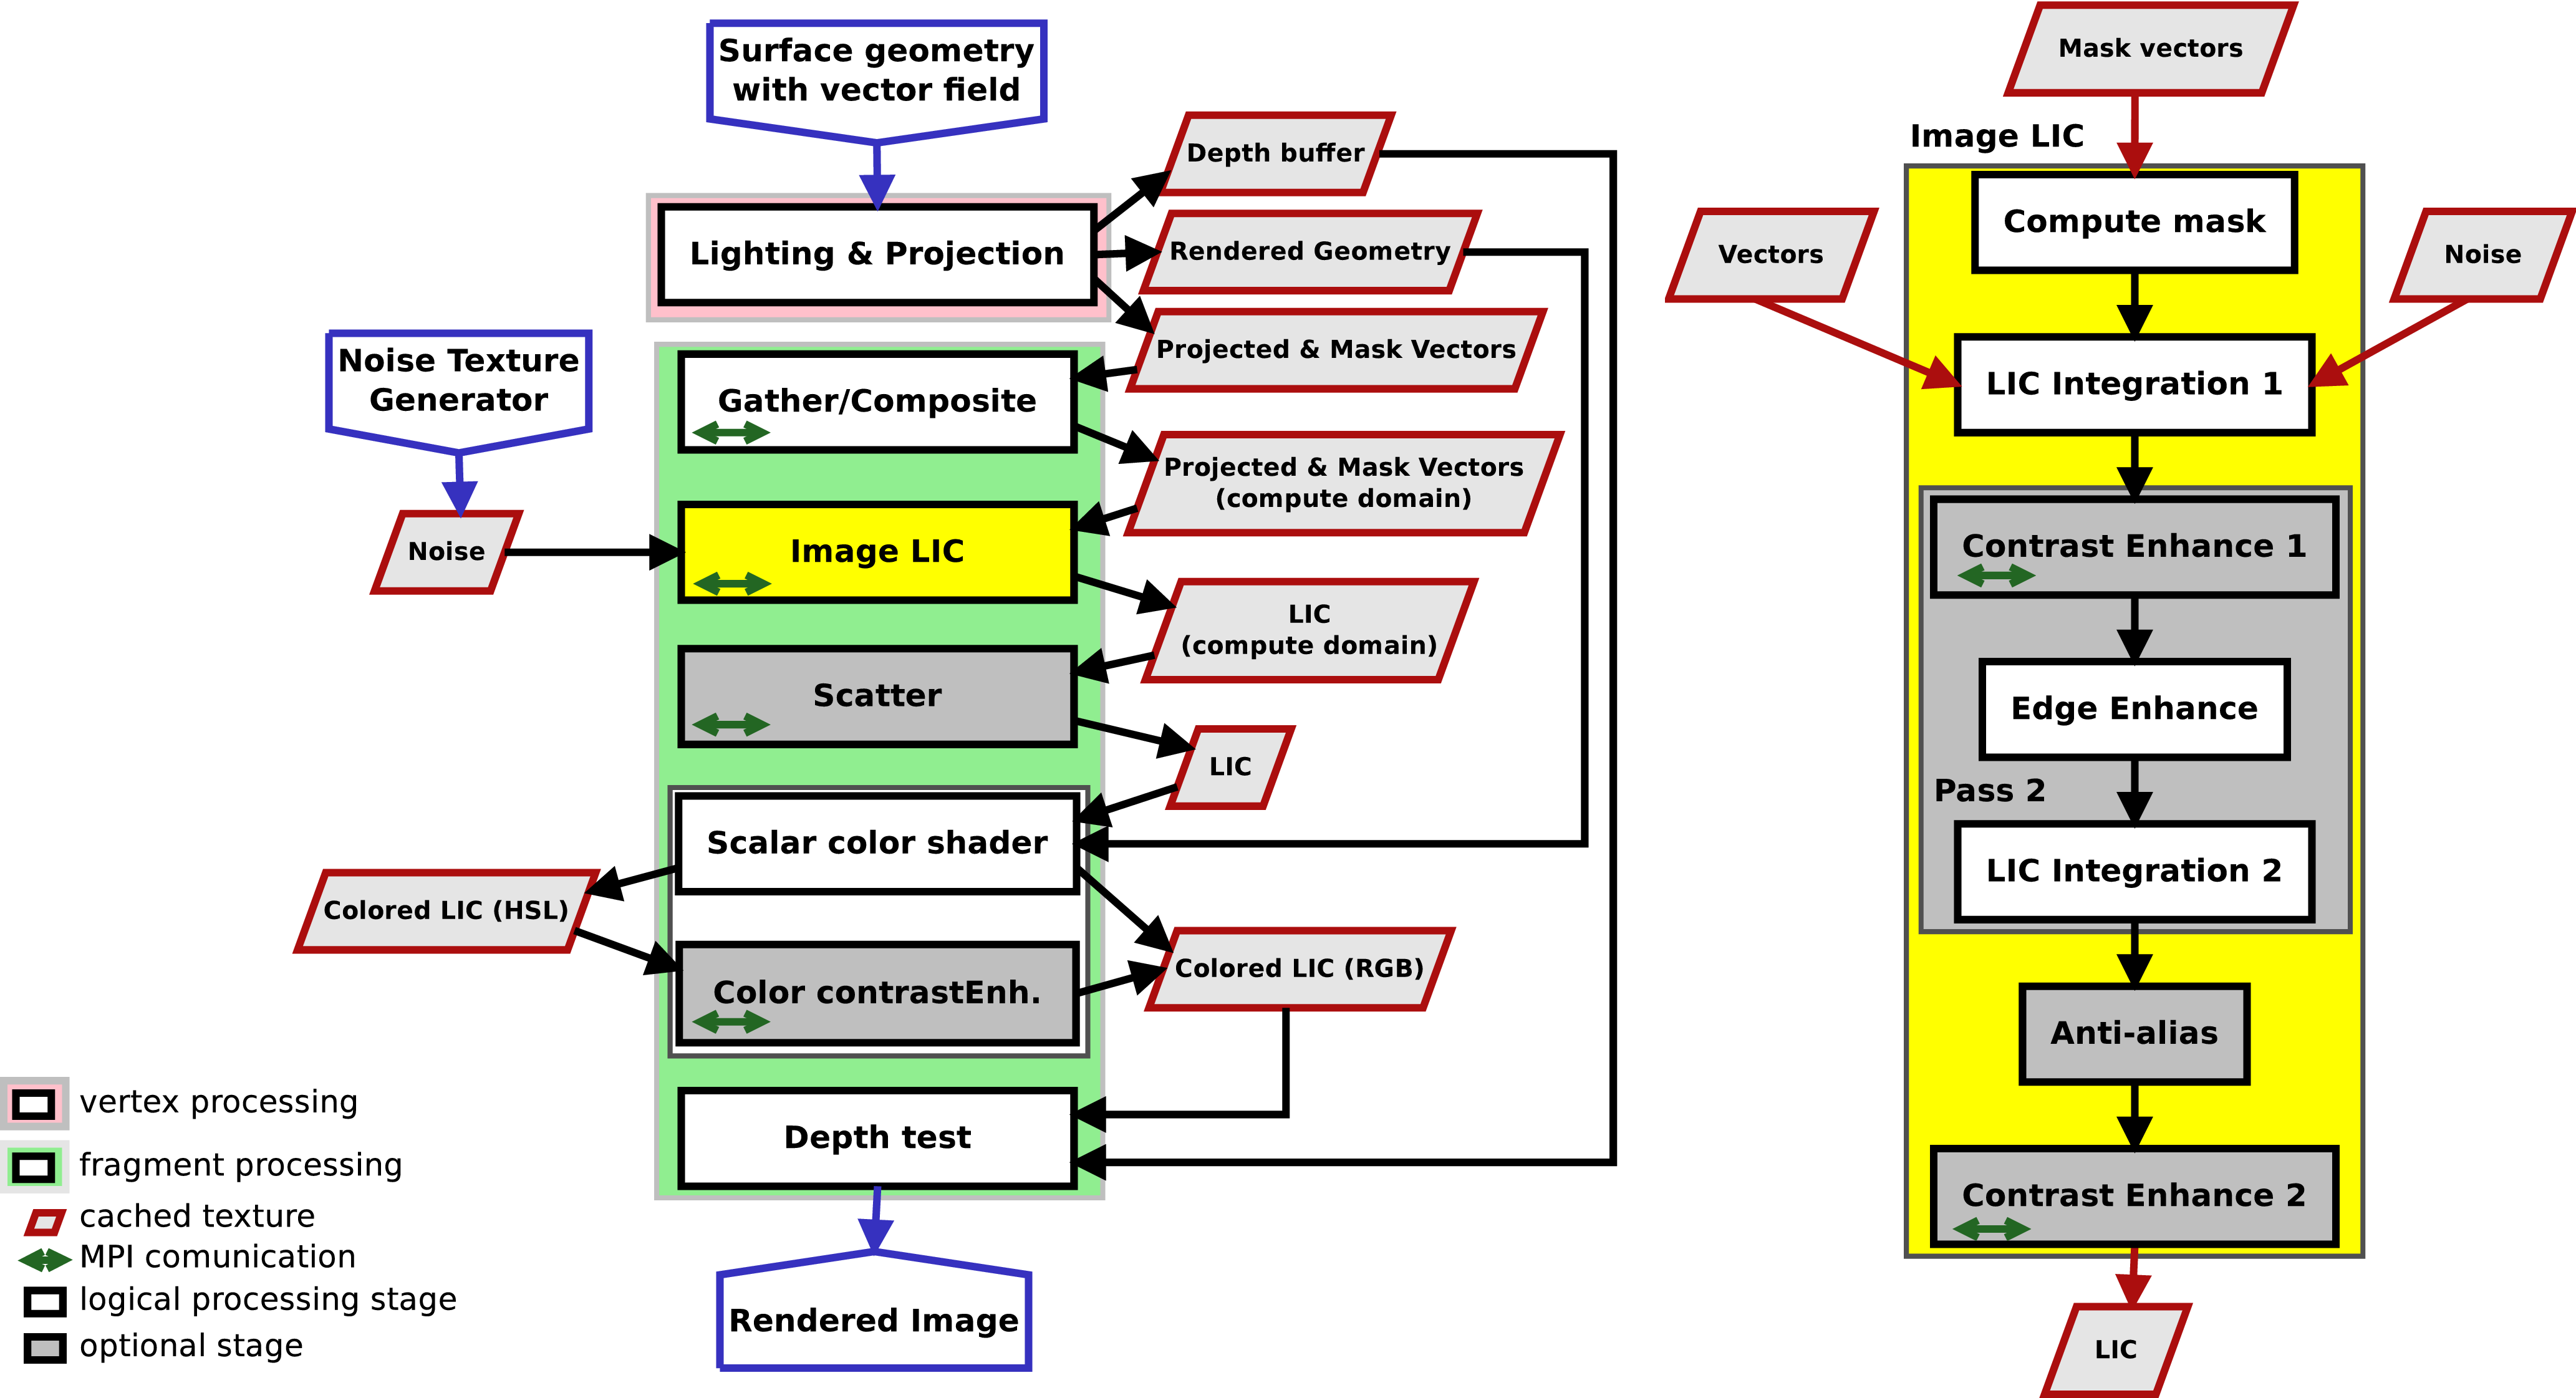
\includegraphics[width=3.75in]{ce-flow.png}}
    \only<2>{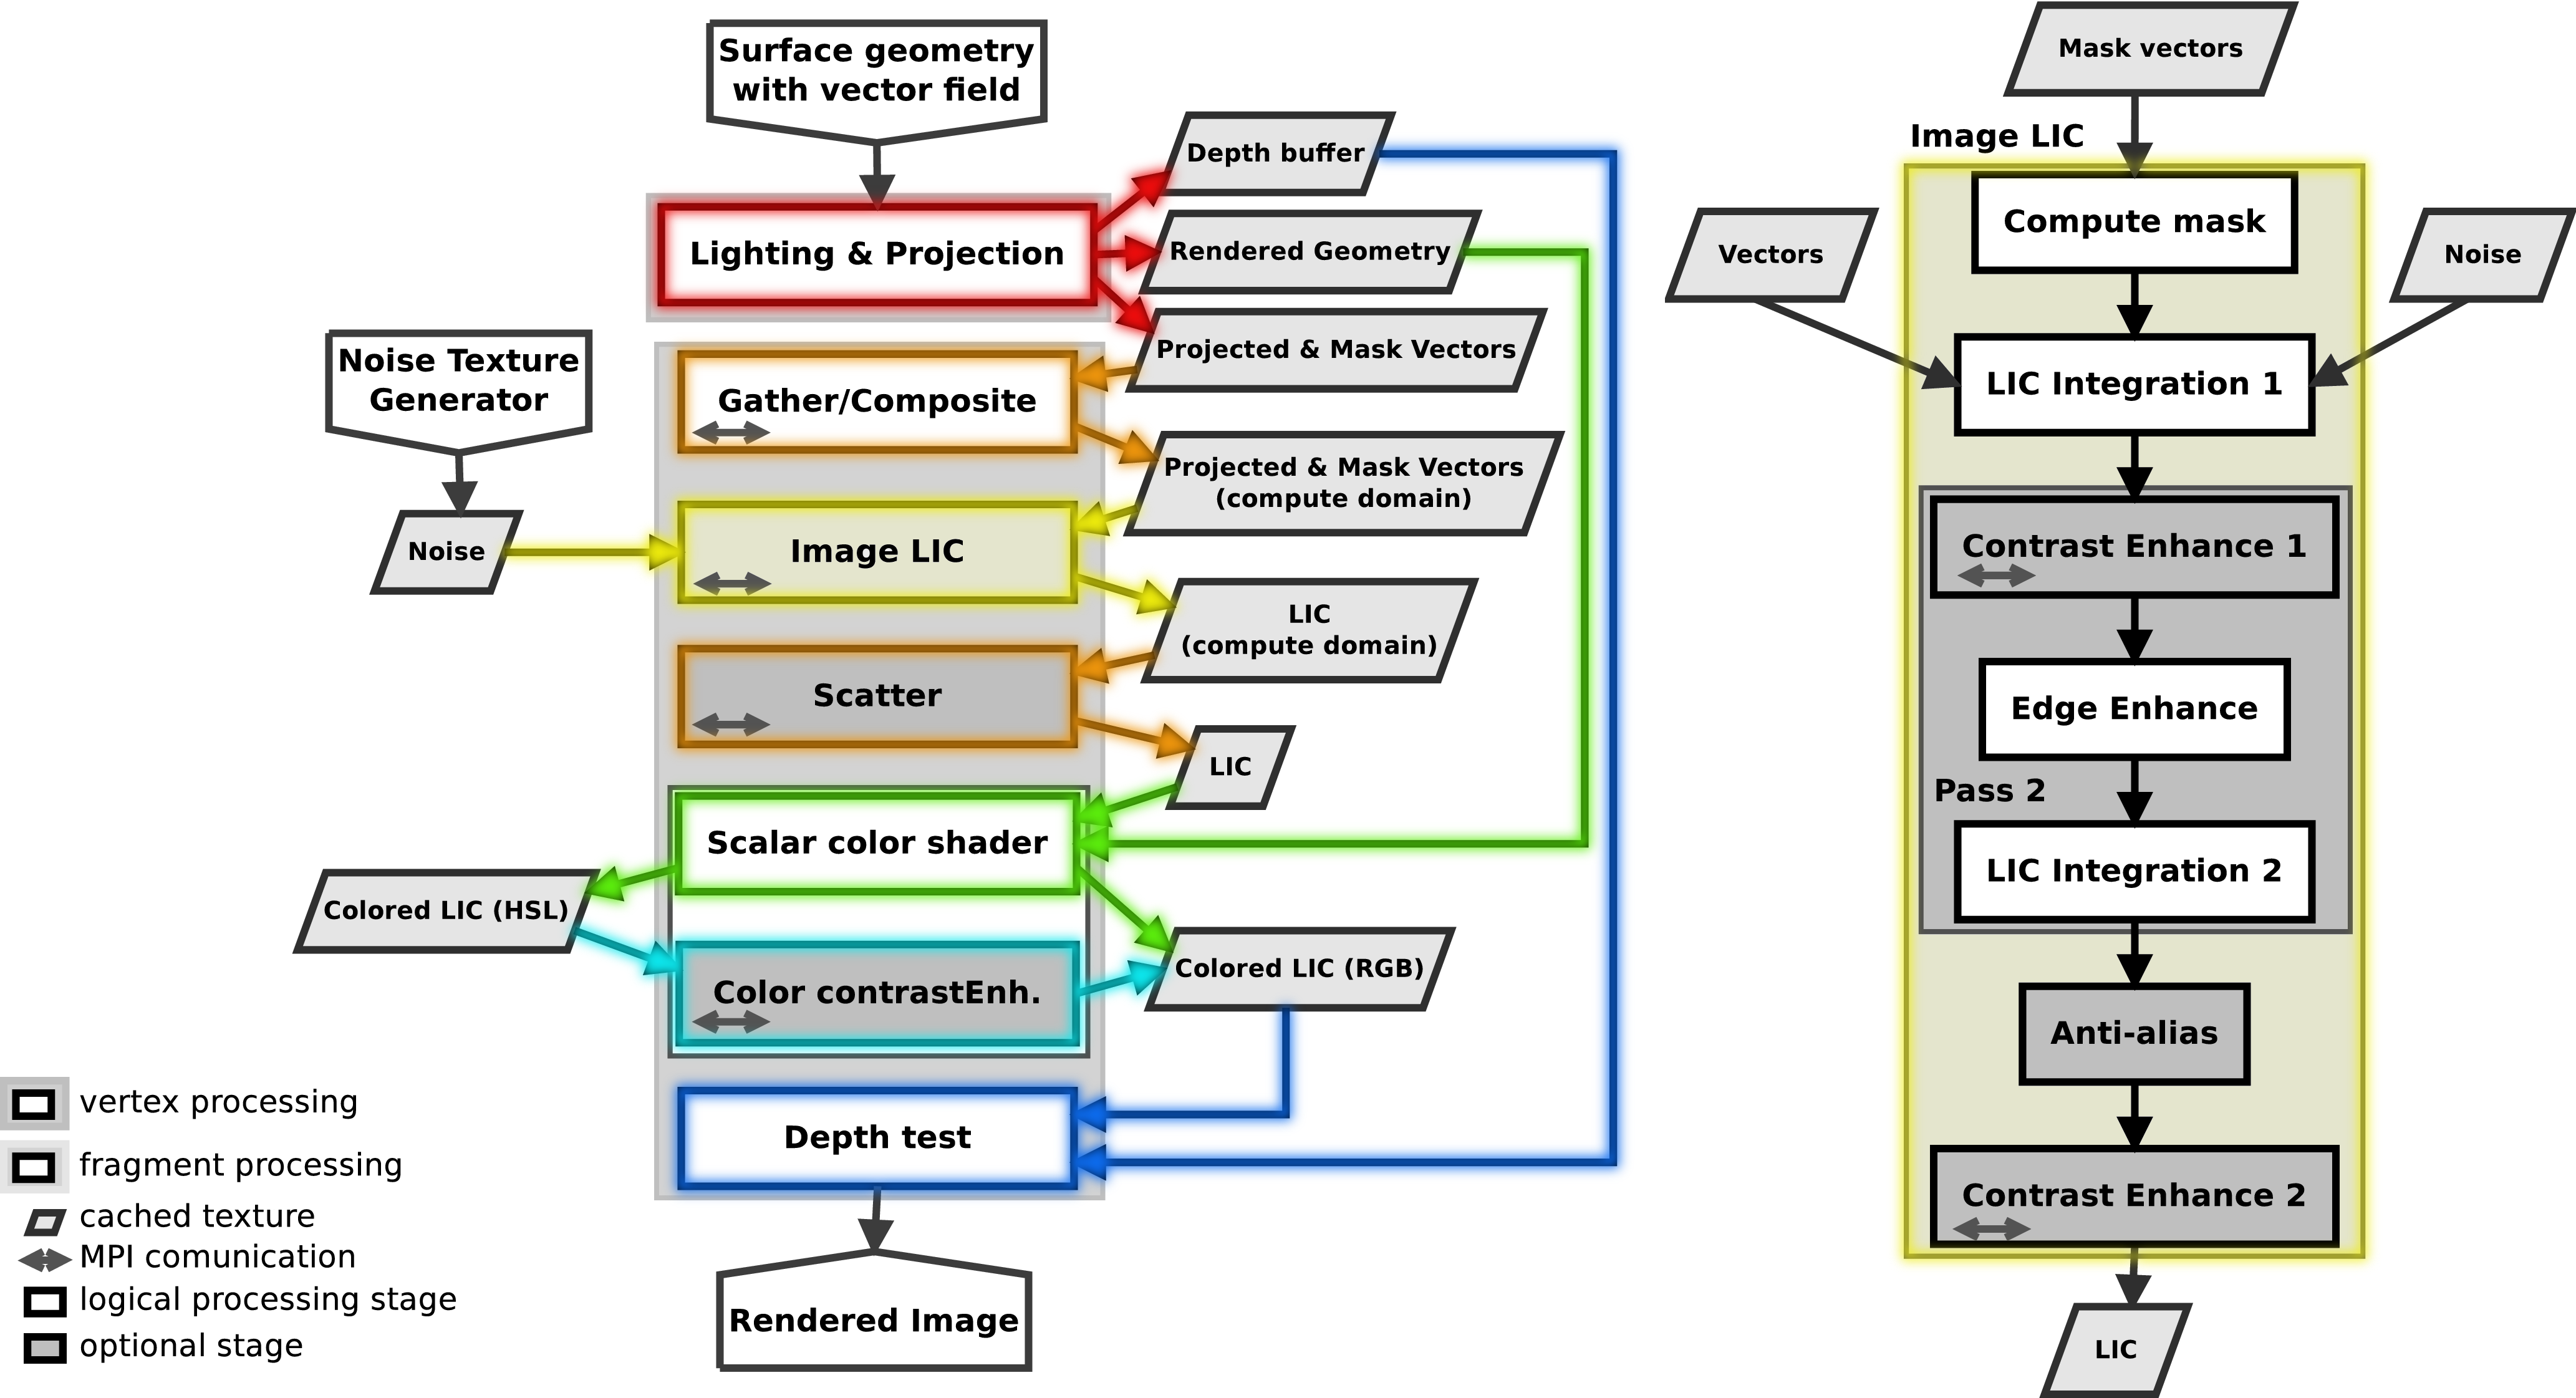
\includegraphics[width=3.75in]{ce-flow-groups.png}
    \begin{itemize}
    \item cache each stage of the pipeline in a texture
    \item group parameters by stage, only run modified and downstream stages
    \end{itemize}
    }
    \end{center}
    \end{minipage}
    \end{beamerboxesrounded}
\end{frame}


%==============================================================================
\begin{frame}{Results}
        \begin{beamerboxesrounded}{What did we accomplish?}
        \begin{minipage}{0.2\linewidth}
        \begin{center}
        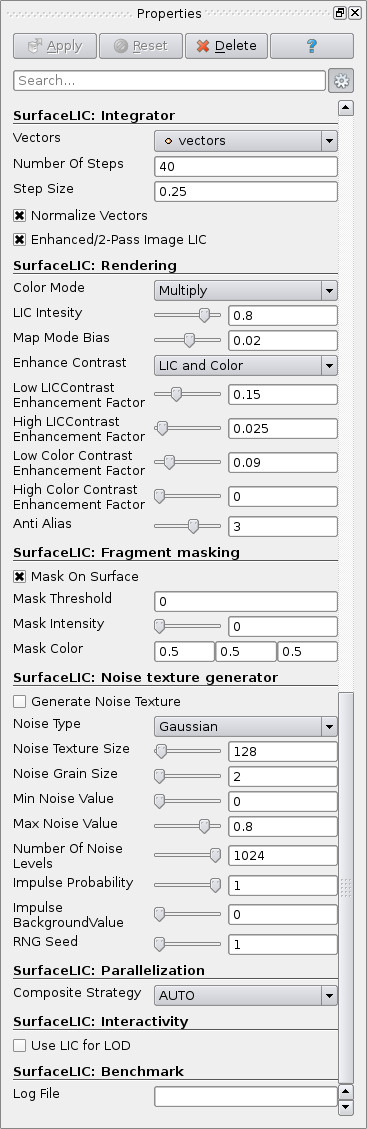
\includegraphics[width=0.9in]{pv-ui.png}
        \end{center}
        \end{minipage}
        \begin{minipage}{0.75\linewidth}
%         \vspace{-0.1in}
        \begin{center}
        \includegraphics[width=3.5in]{lic-b-427-hr-crop.png}
        \end{center}
        \vspace{-0.1in}
        \begin{enumerate}
        \item Apply image processing techniques to produce high contrast high dynamic range pseduocolored results $\Leftrightarrow$ capture fine details and accurately represent the vector field
        \item Expose many knobs $\Leftrightarrow$ Choices are left to runtime in order to effectively deal with data, view, and surface variablity
        \item Optimzations for interaction $\Leftrightarrow$ make interaction practical
        \item Parallelizaiton $\Leftrightarrow$ process very large datasets
        \item Deployment in ParaView
        \end{enumerate}
        \end{minipage}
      \end{beamerboxesrounded}
\end{frame}
\end{document}
